The first step of our approach is Amodal-net, an amodal framework illustrated in \ref{fig:pipeline} without the red annotations. The next step is to try to incorporate 3D information into the data used for training, as shown in red annotations in \ref{fig:pipeline}. Intuitively,  incorporating 3D information should allow the learning pipeline to use the temporal information better. For example, if the pipeline can see that an object is partialy blocked by an object that has a z value, it should know to still map out the object in its whole shape in the amodal mask. 

The SAILVOS dataset\cite{hu2019sail} have annotations for depth map. SAIL-VOS 3D also from Hu \etal \cite{HuCVPR2021} also has camera intrinsics and extrinsics stored in the object files. Although there are some scene mismatches in the unit of a few mili-seconds, I will use these annotations to do mask reprojections in the data training pipeline.

\section{Overview}
Given a sequence of $T$ images $\mI_{t-T:t}=(\mI_{t-T+1}, \hdots, \mI_{t})$ our goal is to predict for each object $o\in\gO_t$ in the current frame $\mI_t$ the corresponding amodal mask $\mM_{t,o}$. 
%set of amodal segmentation masks, \ie, $\gM = \{\mM_{t,o}~\forall o \in \gO_t\}$, where $\mM_{t,o}$ is the amodal mask for object $o\in\gO_t$ in the $t^\text{th}$ frame $\mI_t$, and 
We let $\gO_t$ denote the set of detected objects in frame $\mI_t$, while $\gM_t = \{\mM_{t,o}~\forall o \in \gO_t\}$ refers to the set of segmentation masks.

To accomplish this goal, we first extract features $\phi_t$ for all $T$ frames in $\mI_{t-T:t}$. %We then use
Next, reprojection is used to spatially align features with the current frame $\mI_t$ via warping. We then perform spatial and temporal aggregation to compute the feature $\Phi_t$. This ensures that the backbone feature $\Phi_t$ summarizes temporal information. 

Next, our cascade Soft-NMS box-head detects objects and crops $\Phi_t$ to extract object-level features $\Phi_{t,o}$ for each detected object $o\in\gO_t$. Our box-head uses soft-thresholding during non-maximum suppression to better handle overlapping boxes. Given the object-level features $\Phi_{t,o}$, the amodal mask $\mM_{t,o}$ for each object is predicted using an iterative mask-head. We incorporate a large receptive field and self-attention into the iterative mask-head. % using a large receptive field and self-attention. 
Because of this, information can propagate across the entire detection during mask prediction.

\section{Amodal-Net}
The base model is Amodal-Net builds on top of Mask R-CNN\cite{he2017mask}. Given the candidate bounding boxes, ROIAlign~\cite{he2017mask} is used to extract a feature map for each of the candidate boxes. The bounding box features are subsequently processed by a box-head and/or a mask-head, which regress to bounding box and segmentation mask respectively. The box-head consists of fully connected layers and yields a classification prediction and a  corresponding bounding box.  %the bounding box size and its location. 
The mask-head consists of a stack of convolutional layers. 

Variants of Mask-RCNN rely on a multi-stage refinement approach, \ie, a cascade is used to enhance the box-prediction accuracy~\cite{cai2018cascade, chen2019hybrid}. While our method also relies on a cascade design, our model is specifically designed for the task of SAIL-VOS. Amodal-net that Yeh and I developed with collaborator uses a temporal backbone to aggregate information over time, Soft-NMS to handle overlapping amodal boxes, and an iterative mask-head with attention to propagate information into occluded regions, as shown in \ref{fig:pipeline}. We also found that multi-task training with the occlusion prediction task further improves performance. Combining the aforementioned techniques results in the following framework, for which a pictorial sketch is shown in~\figref{fig:pipeline}. This multi-task training is only included in the experiments for the Amodal-net and not included in the experiments with 3D Reprojection due to limitations in computation resources.

The changes in Amodal-net is made to address three challenges in this task: {\bf (i)} a limited use of temporal information; {\bf (ii)} a missing mechanism to handle heavily overlapping amodal boxes; and {\bf (iii)} 
a propagation of object observations which is often too short-sighted. Amodal-net is based on {\bf (i)} a  temporal backbone which aggregates information across video frames, {\bf (ii)} a box-head which 
better adjusts to overlapping detection boxes by using a cascade architecture with  Soft-NMS, 
and {\bf (iii)} a mask-head with increased receptive field and self-attention to propagate observations more broadly. Each of these components addresses the corresponding  challenge. 



\section{3D Reprojection}
Following the aforementioned intuition, 3D reprojection is added in the pipeline to align inputs in the temporal dimention, as shown in red in \ref{fig:pipeline}. In the input, along with the images from $t$ and $t-1$ frames, the camera matrices and the depth map of the corresponding frames is also passed in. The camera matrices include the intrinsic and extrinsic matrices of the camera.

The depth map and the camera matrices together is used to do reprojections from one frame to another. Standard computer vision reprojection algorithm warps an image from the perspective of one image to the perspetive of another image.

Given the image and the depth value of every pixel, we can get the camera coordinates for each pixel $X_{cam}$. For example, \ref{fig:3Dproj} plots one image in camera coordinates in 3D. Then it is possible to calculate the camera coordinates of every pixel in another frame by using the camera matrices. $$ X_{cam} = K[R|t]X_{world} $$ where $K$ is the intrinsic matrix and $[R|t]$ is the extrinsic matrix representing rotation and translation of the camera. If we have two cameras looking at the same scene, $$X_{cam2} = K_2[R_2|t_2](K_1[R_1|t_1])^{-1}X_{cam1}$$ Finally, we can use $X_{cam2}$ to recover the pixel coordinates and thus get the reprojected image in 2 dimensions. One complication in implementation is that initially I wasn't sure what format the depth map is stored in. After consulting with authors of \cite{hu2019sail} and some exploration, I discovered that the data is stored in a variation of NDC format. So camera coordinates of the image $X_{cam}$ had to be computed from NDC coordinates $X_ndc$. The details of the implementation is \ref{apx:reproj}. 

I also experimented with estimating the camera matrices from 2D and 3D points correspondence. However, due to the nature of how the data is collected in GTA-V and the format of the depth map. The estimated camera matrices induces a large error in reprojection compared to groundtruth camera matrices. In the end, I decided to use the groundtruth matrices recorded. 

We can perform reprojeciton in image frames or masks. \ref{fig:reproj_image} shows an example of the reprojected image frame in full, and \ref{fig:reproj_mask} shows some examples of reprojected masks. In these plots, the first picture is the groundtruth image of frame $t$; the second picture is the groundtruth image of frame $t-2$; the third picture is the groundtruth mask of an object at frame $t$; the fourth picture is the mask of the object at $t-2$ reproject into the perspective of frame $t$; the last picture of the mask of the object at frame $t-2$ directly. The caption shows intersection over union of the last two masks with the groundtruth mask \ie the third mask. The reprojected image and mask should provide accurate information of the scene in previous frames since reprojection compensates the movement of the camera. But there is one drawback of this approach: it does not take into account the movement of objects in the scene. If the object is also moving, the reprojected image would not reflect that. But we can see from the captions of \ref{fig:reproj_image}, in general reprojected mask is closer to the groundtruth mask than directly using the mask from another frame, especially for objects that are still. 

In the network, we use the same algorithm but perform reprojection on the features of images produced by the backbone. By doing so, the features from different temporal indices are aligned in the sense that there are from the same perspective, and each pixel corresponds to the same spatial location. For this purpose, the depth map is reshaped into different shapes in the network to match the dimension of the features in the feature pyramid.

\begin{figure}

\centering
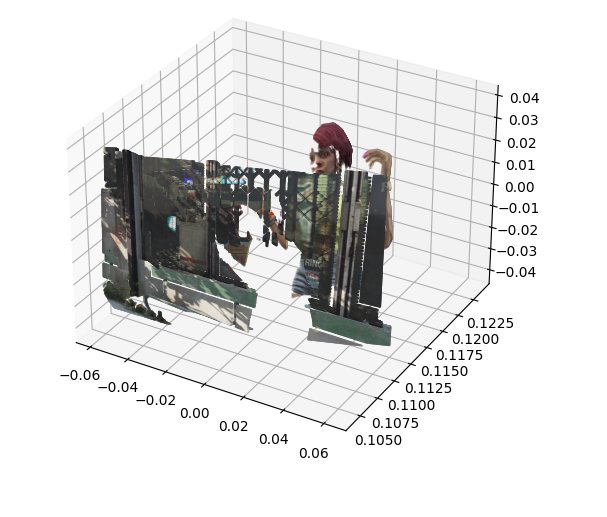
\includegraphics[scale=0.5]{fig/3dproj.png}
\caption{Projection of a frame in 3D camera coordinates}
\label{fig:3Dproj}
\end{figure}


%\begin{figure}
\centering
\begin{subfigure}[t]{0.19\textwidth}
\centering
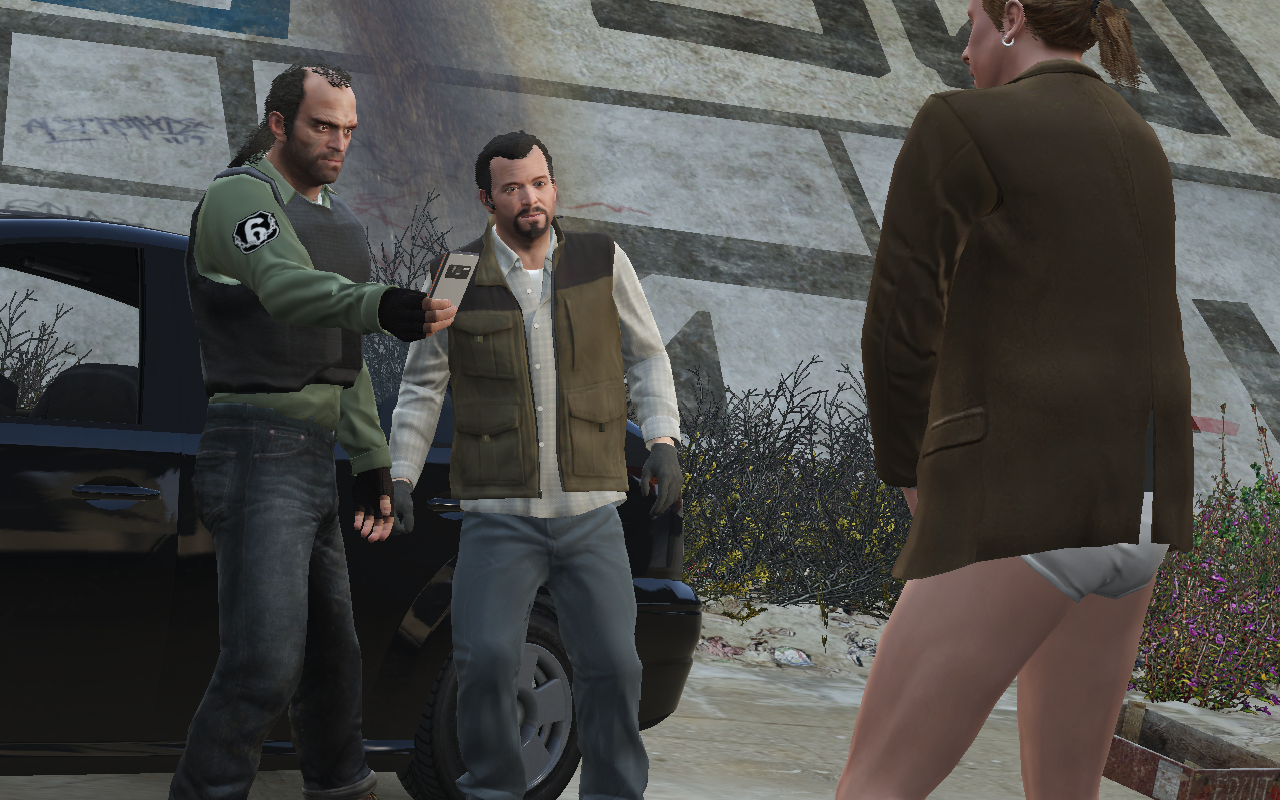
\includegraphics[scale=0.07]{good_examples/visual_179486_img.png}
\end{subfigure}
\begin{subfigure}[t]{0.19\textwidth}
\centering
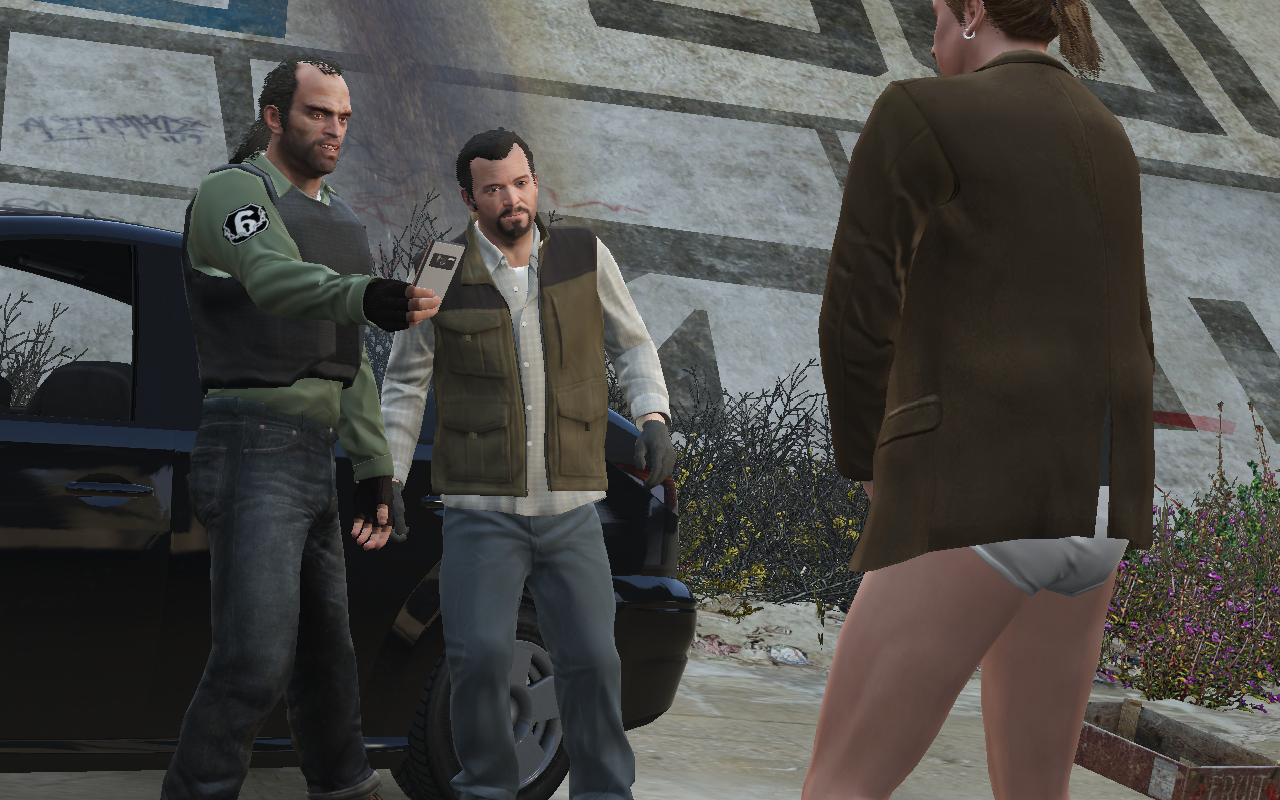
\includegraphics[scale=0.07]{good_examples/visual_179486_img1.png}
\end{subfigure}
\begin{subfigure}[t]{0.19\textwidth}
\centering
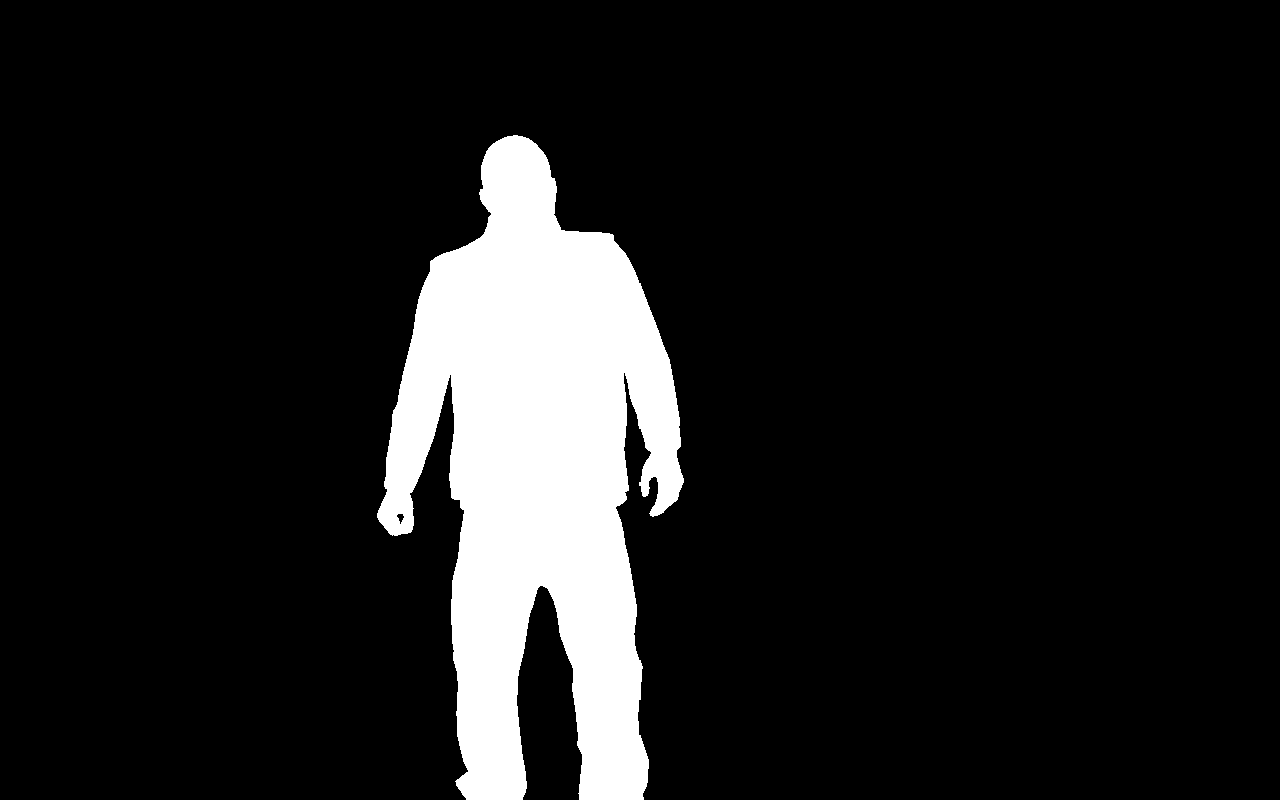
\includegraphics[scale=0.07]{good_examples/visual_179486_gt.png}
\end{subfigure}
\begin{subfigure}[t]{0.19\textwidth}
\centering
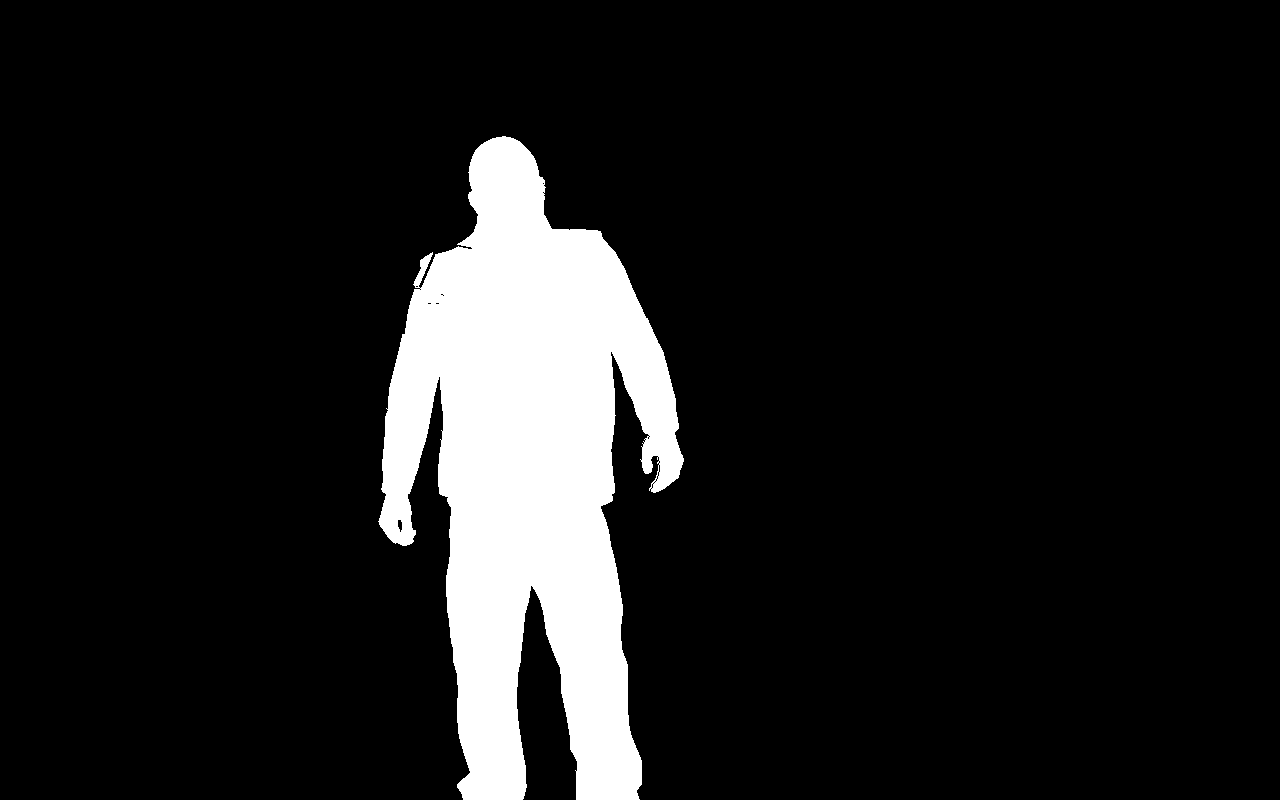
\includegraphics[scale=0.07]{good_examples/visual_179486_w_np.png}
\end{subfigure}
\begin{subfigure}[t]{0.19\textwidth}
\centering
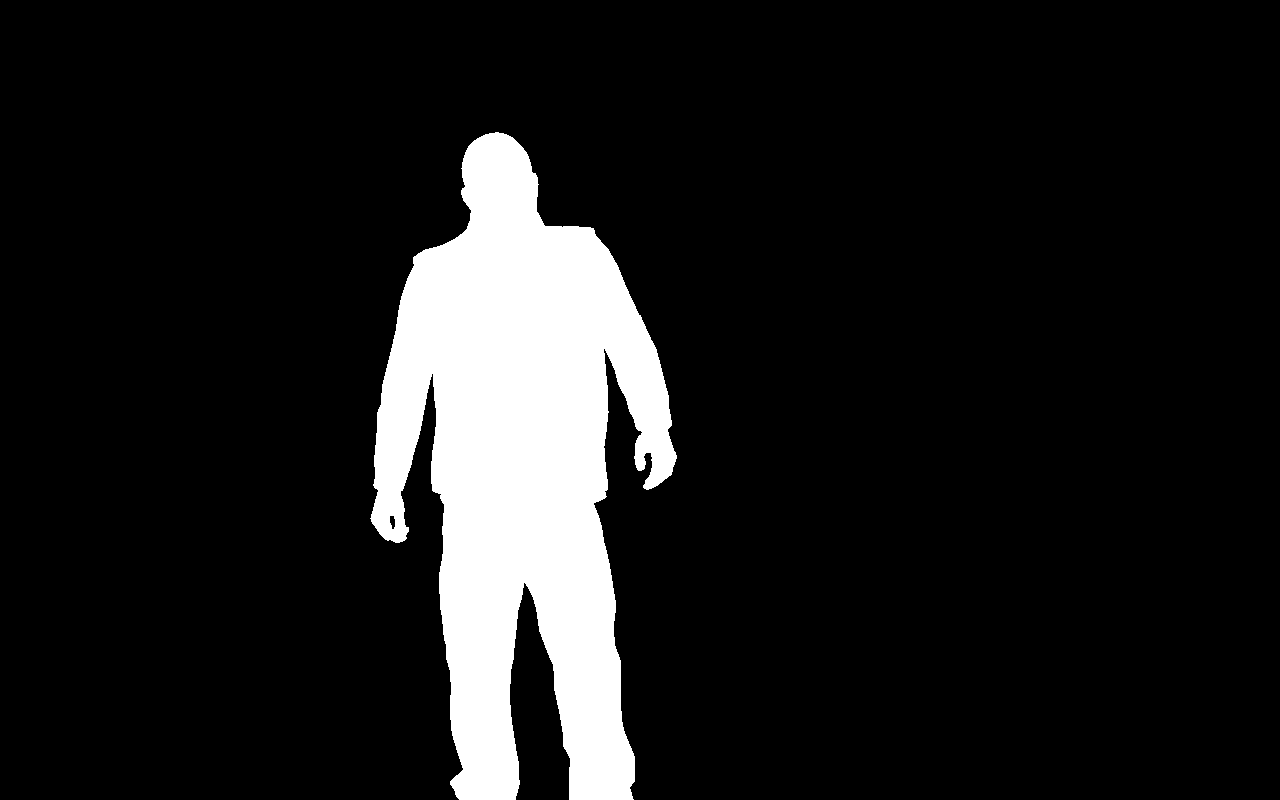
\includegraphics[scale=0.07]{good_examples/visual_179486_wo_np.png}
\end{subfigure}
\caption{IOU with reprojection: 0.85, IOU without reprojection: 0.75, video\_name: family\_4\_mcs\_3\_concat, frame\_number: 605.}
\label{fig:reproj_mask}
\end{figure}

\begin{figure}
\centering
\begin{subfigure}[t]{0.19\textwidth}
\centering
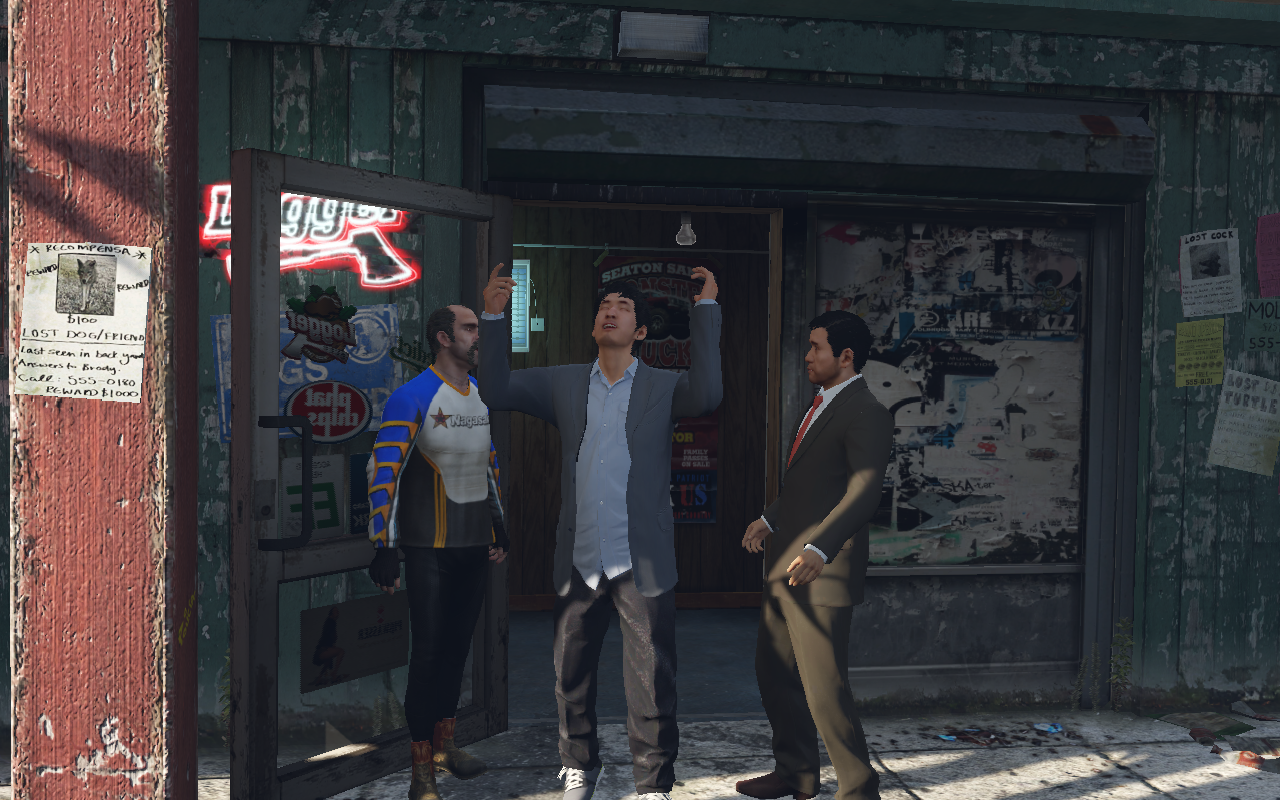
\includegraphics[scale=0.07]{good_examples/visual_74577_img.png}
\end{subfigure}
\begin{subfigure}[t]{0.19\textwidth}
\centering
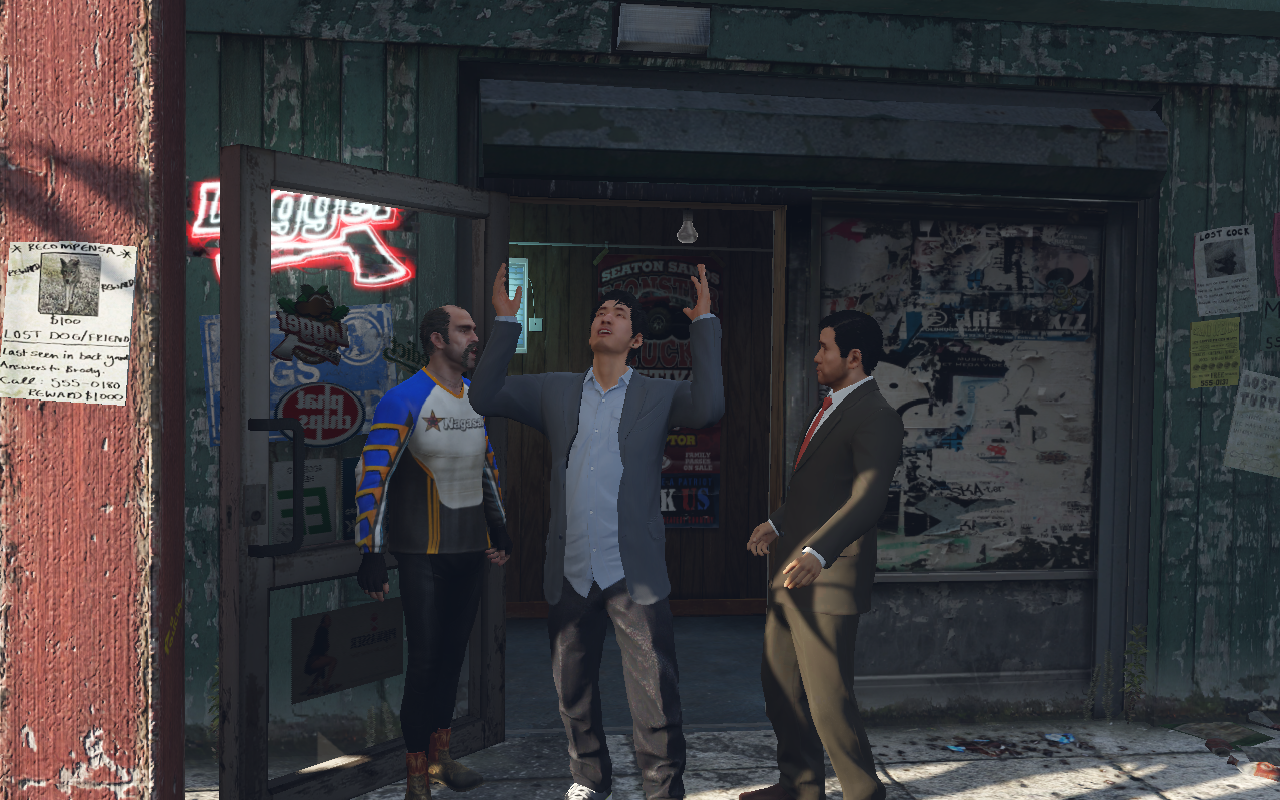
\includegraphics[scale=0.07]{good_examples/visual_74577_img1.png}
\end{subfigure}
\begin{subfigure}[t]{0.19\textwidth}
\centering
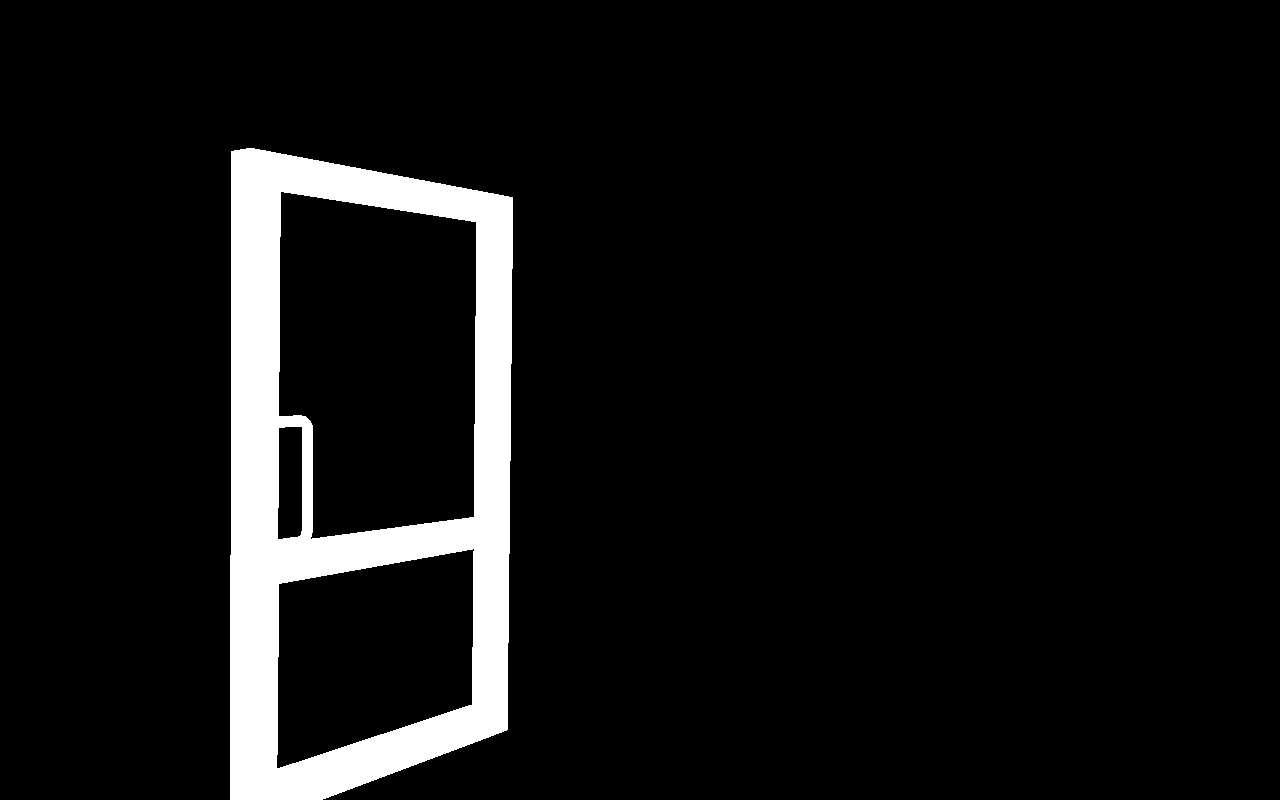
\includegraphics[scale=0.07]{good_examples/visual_74577_gt.png}
\end{subfigure}
\begin{subfigure}[t]{0.19\textwidth}
\centering
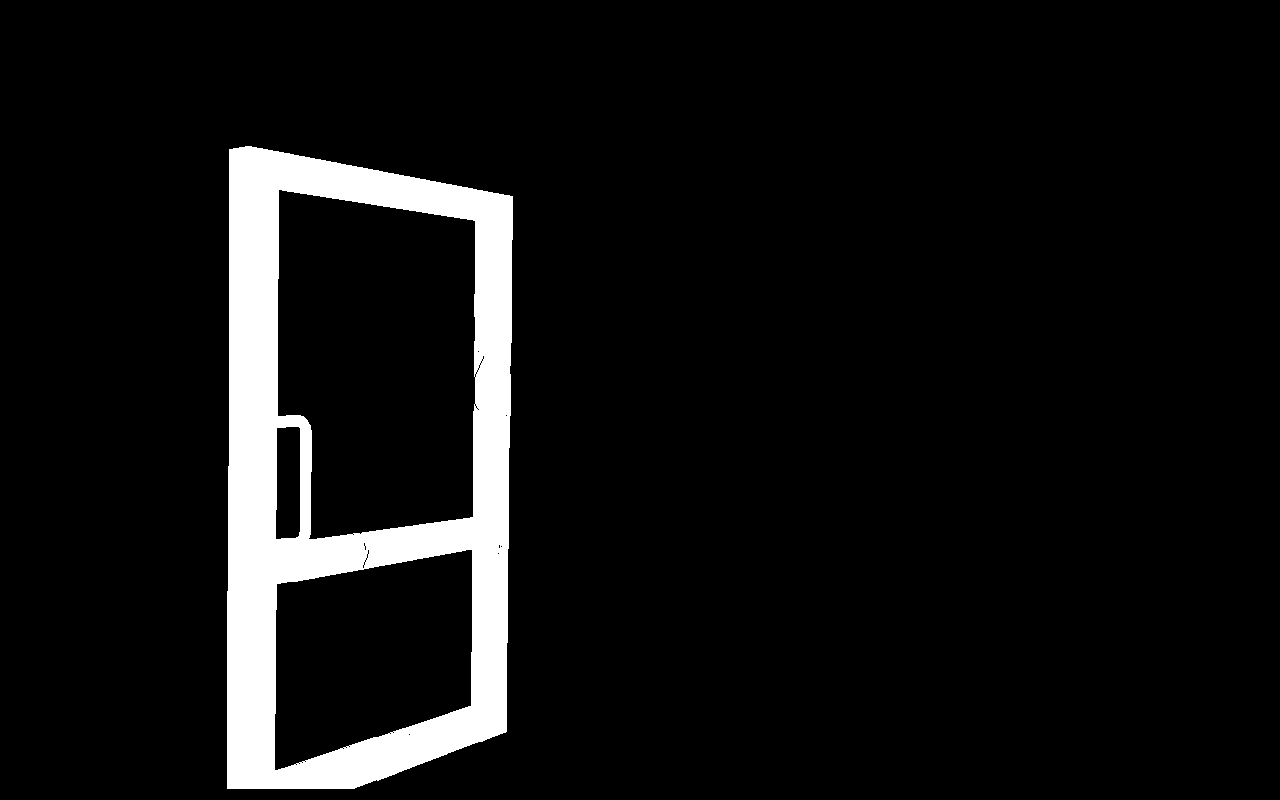
\includegraphics[scale=0.07]{good_examples/visual_74577_w_np.png}
\end{subfigure}
\begin{subfigure}[t]{0.19\textwidth}
\centering
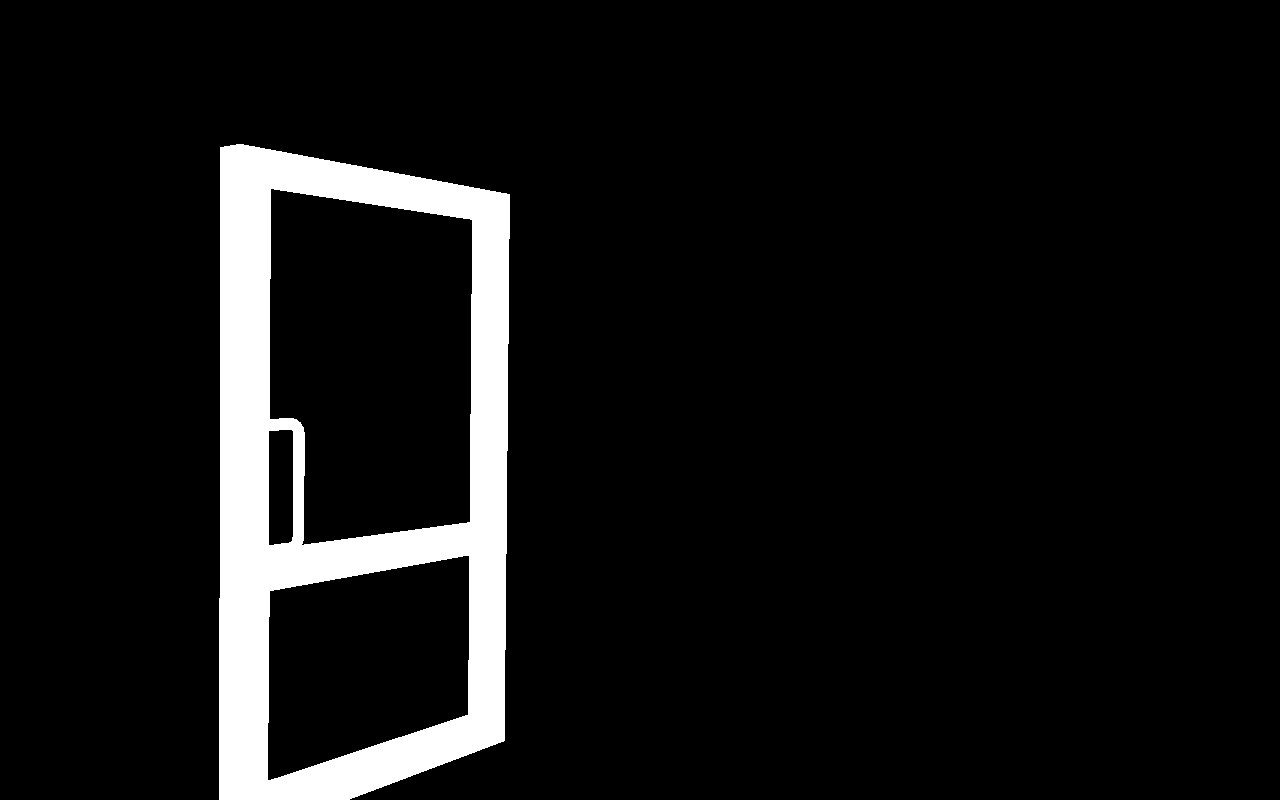
\includegraphics[scale=0.07]{good_examples/visual_74577_wo_np.png}
\end{subfigure}
\caption{IOU with reprojection: 0.91, IOU without reprojection: 0.72, video\_name: chinese\_1\_int, frame\_number: 978.}
\end{figure}

\begin{figure}
\centering
\begin{subfigure}[t]{0.19\textwidth}
\centering
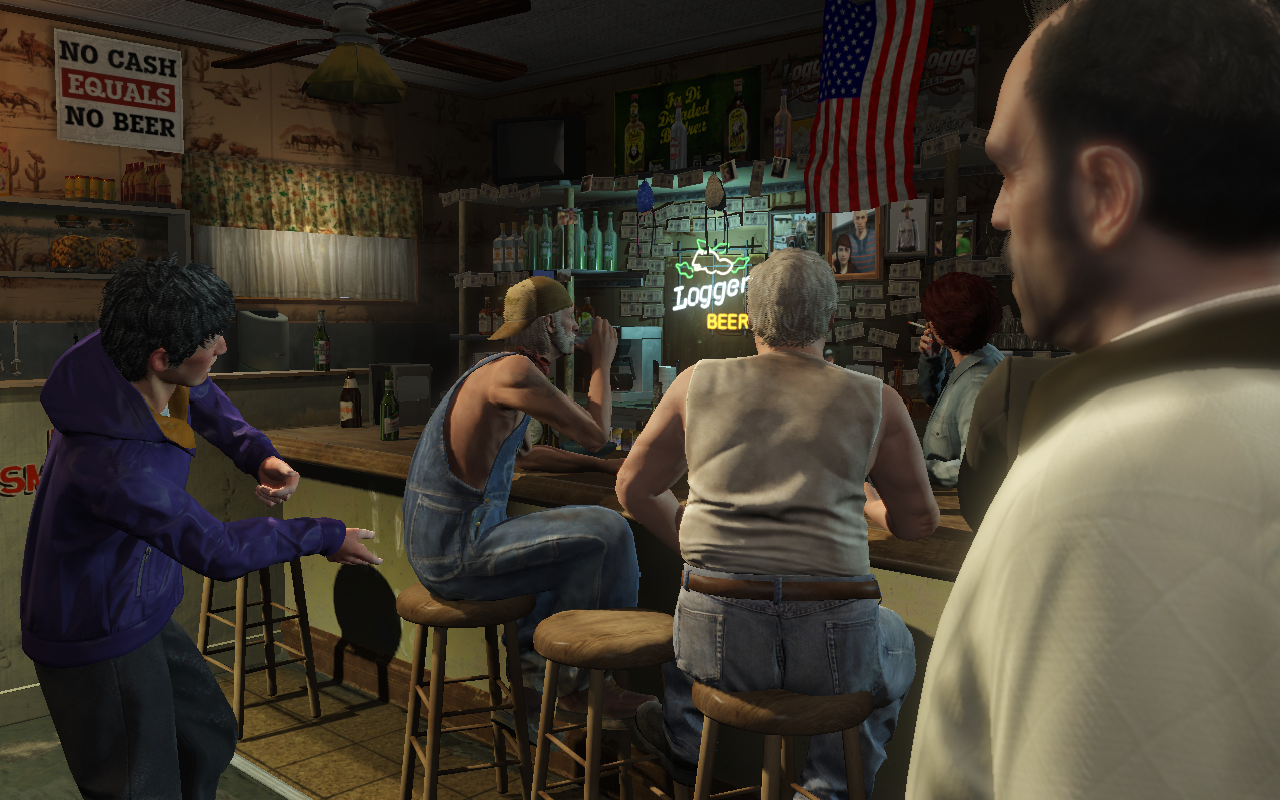
\includegraphics[scale=0.07]{good_examples/visual_76165_img.png}
\end{subfigure}
\begin{subfigure}[t]{0.19\textwidth}
\centering
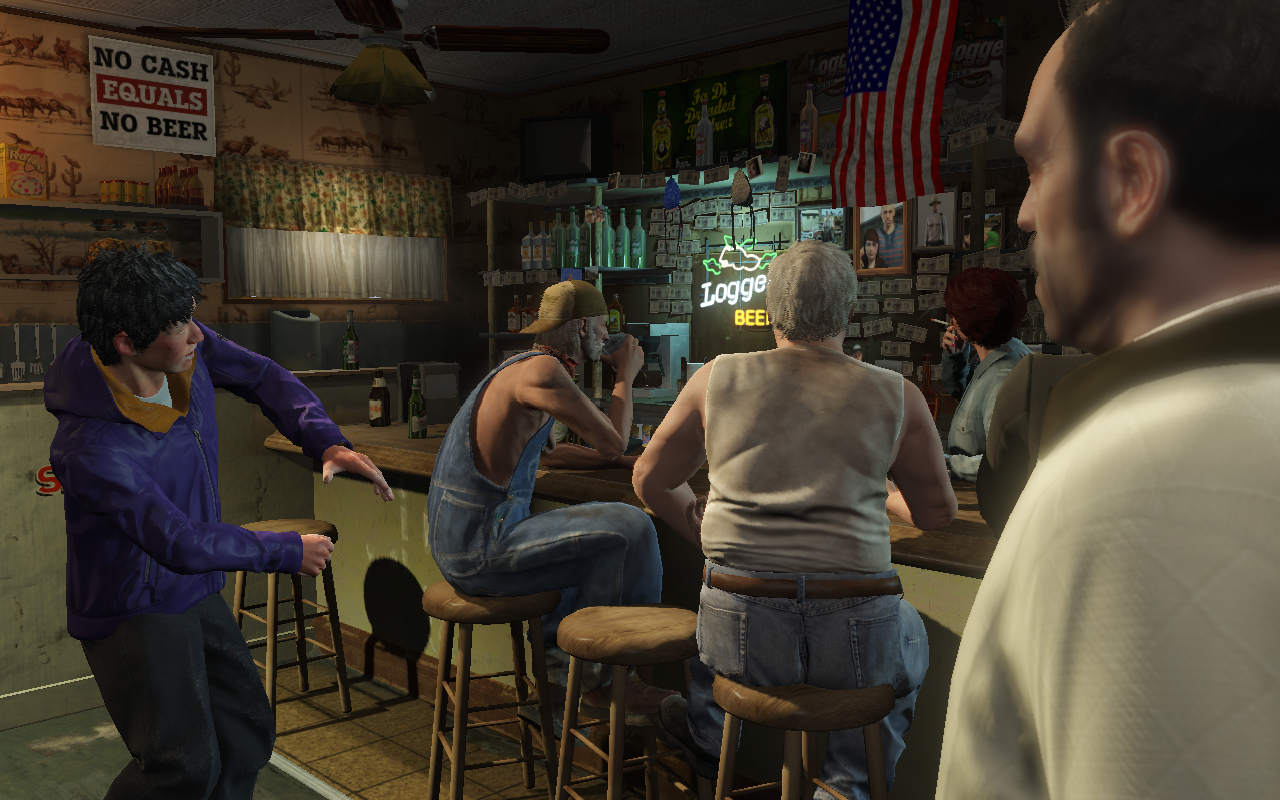
\includegraphics[scale=0.07]{good_examples/visual_76165_img1.png}
\end{subfigure}
\begin{subfigure}[t]{0.19\textwidth}
\centering
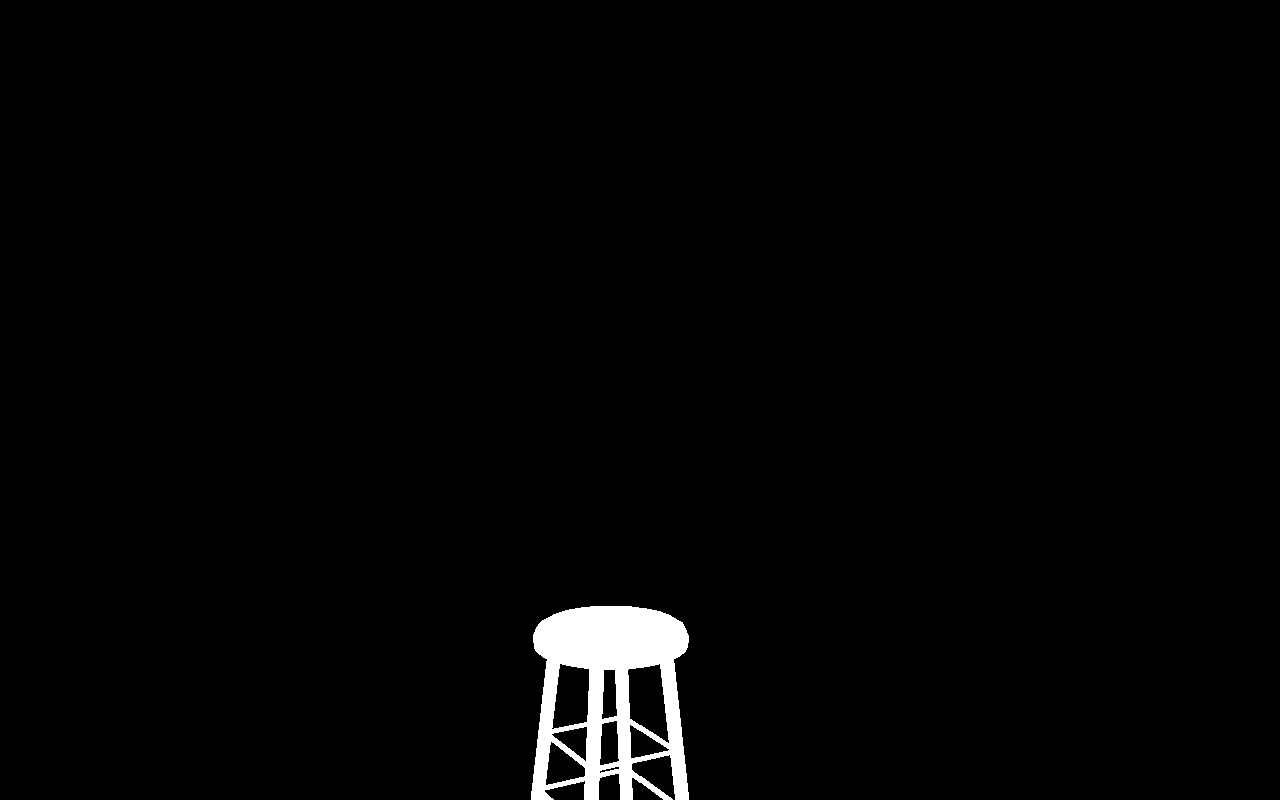
\includegraphics[scale=0.07]{good_examples/visual_76165_gt.png}
\end{subfigure}
\begin{subfigure}[t]{0.19\textwidth}
\centering
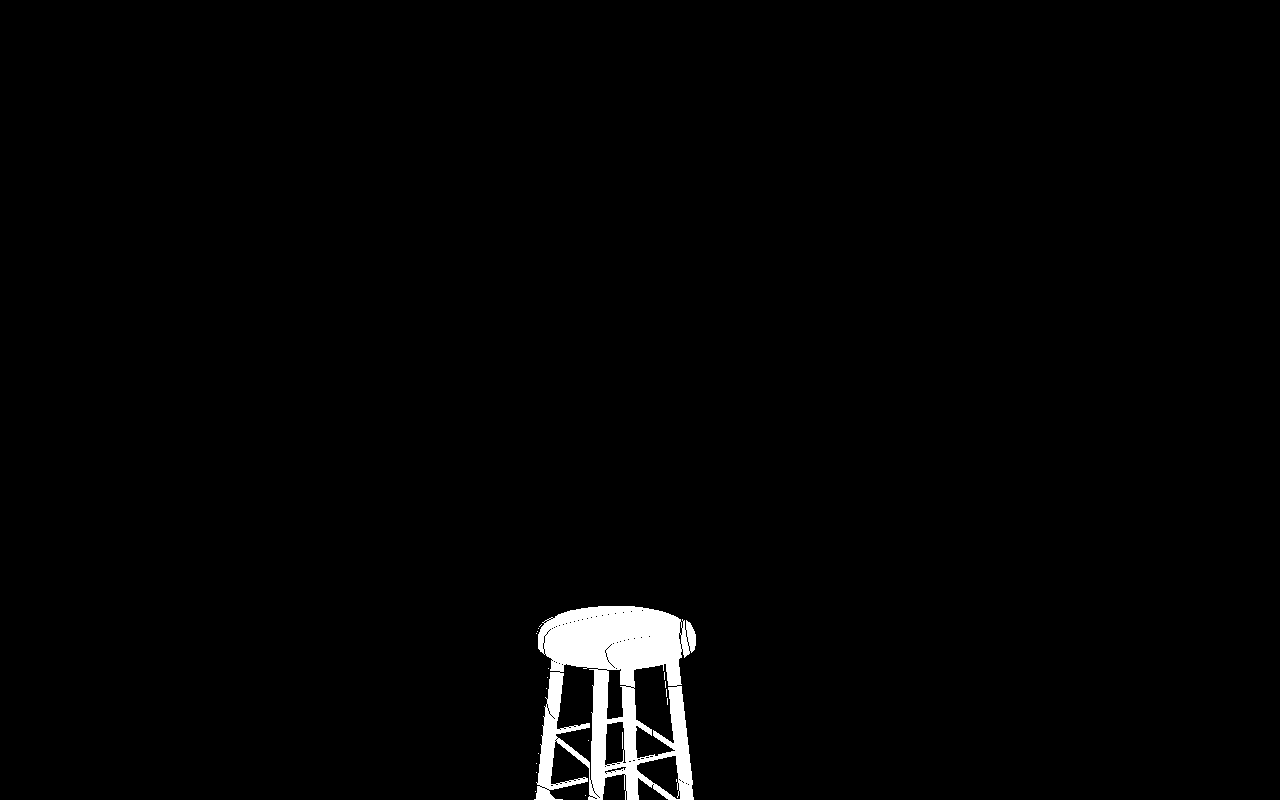
\includegraphics[scale=0.07]{good_examples/visual_76165_w_np.png}
\end{subfigure}
\begin{subfigure}[t]{0.19\textwidth}
\centering
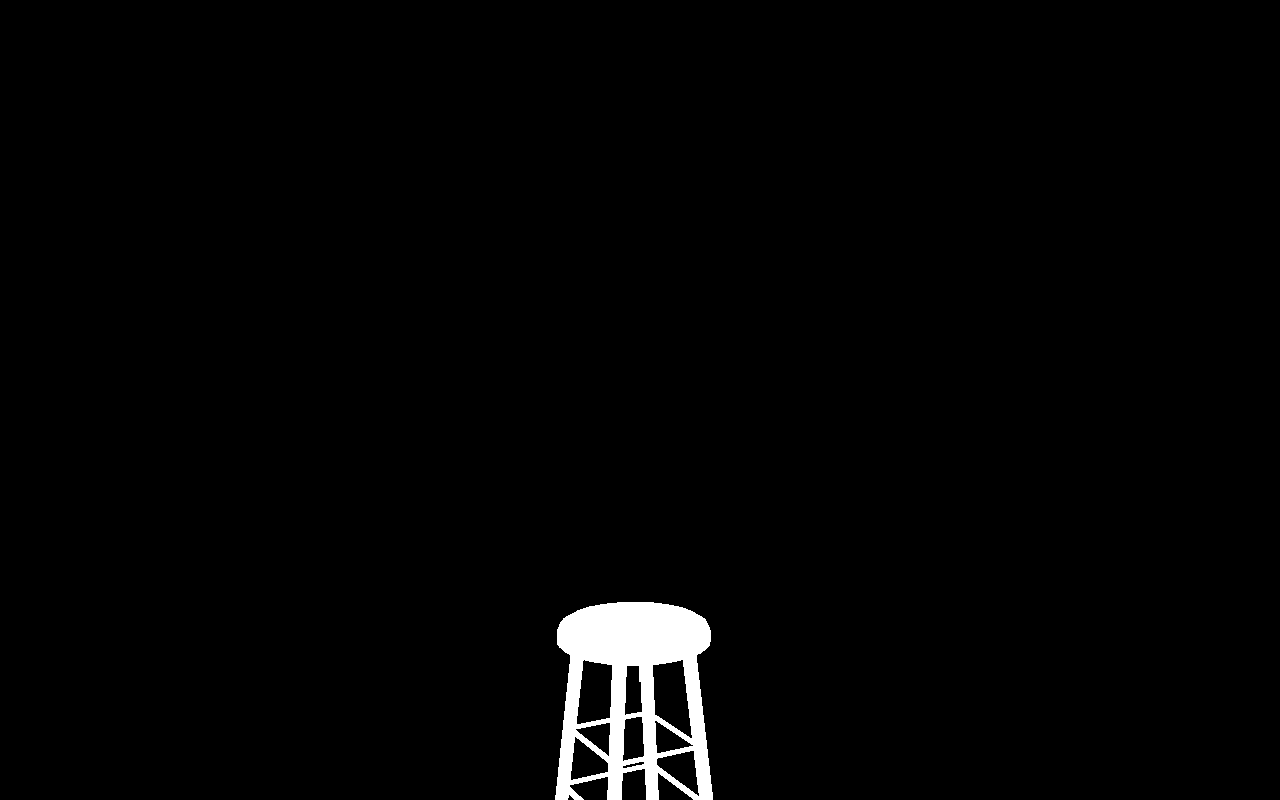
\includegraphics[scale=0.07]{good_examples/visual_76165_wo_np.png}
\end{subfigure}
\caption{IOU with reprojection: 0.67, IOU without reprojection: 0.36, video\_name: chinese\_2\_int, frame\_number: 67.}
\end{figure}


\begin{figure}
\centering
\begin{subfigure}[t]{0.19\textwidth}
\centering
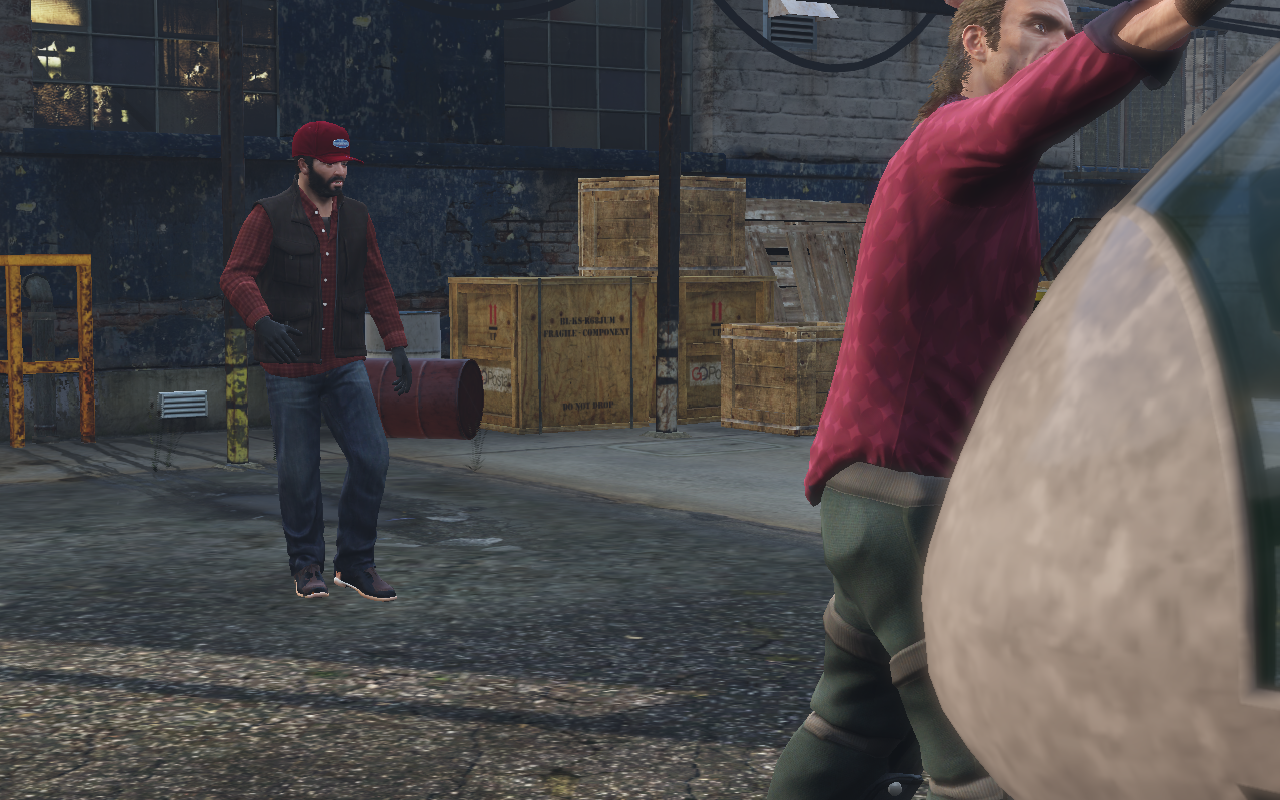
\includegraphics[scale=0.07]{good_examples/visual_211770_img.png}
\end{subfigure}
\begin{subfigure}[t]{0.19\textwidth}
\centering
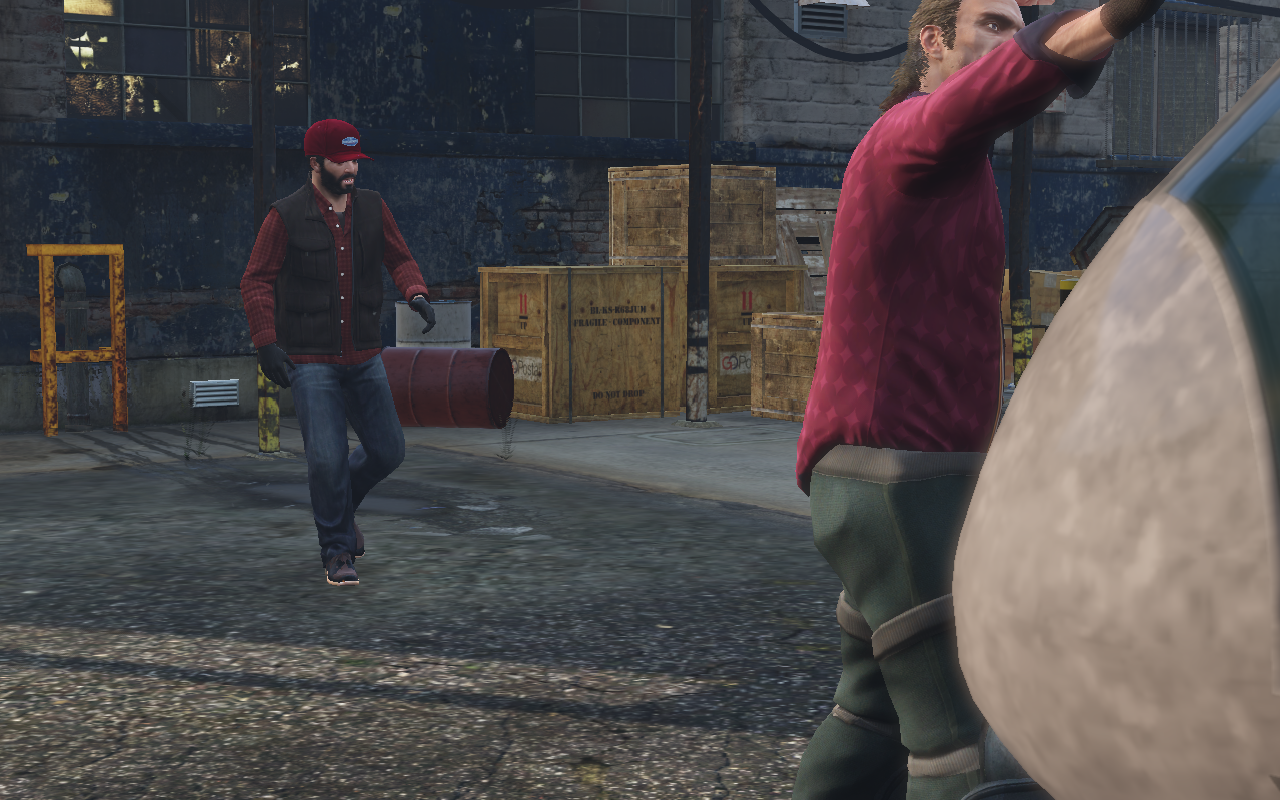
\includegraphics[scale=0.07]{good_examples/visual_211770_img1.png}
\end{subfigure}
\begin{subfigure}[t]{0.19\textwidth}
\centering
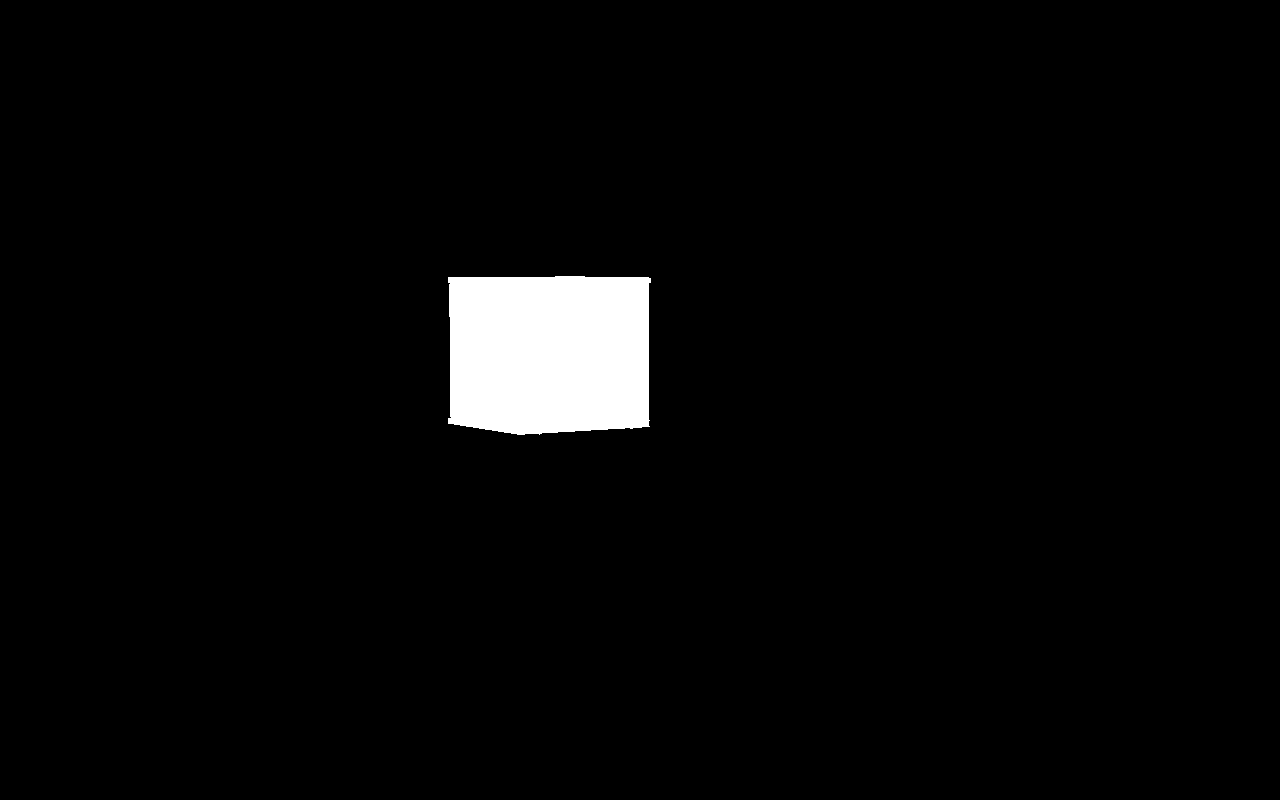
\includegraphics[scale=0.07]{good_examples/visual_211770_gt.png}
\end{subfigure}
\begin{subfigure}[t]{0.19\textwidth}
\centering
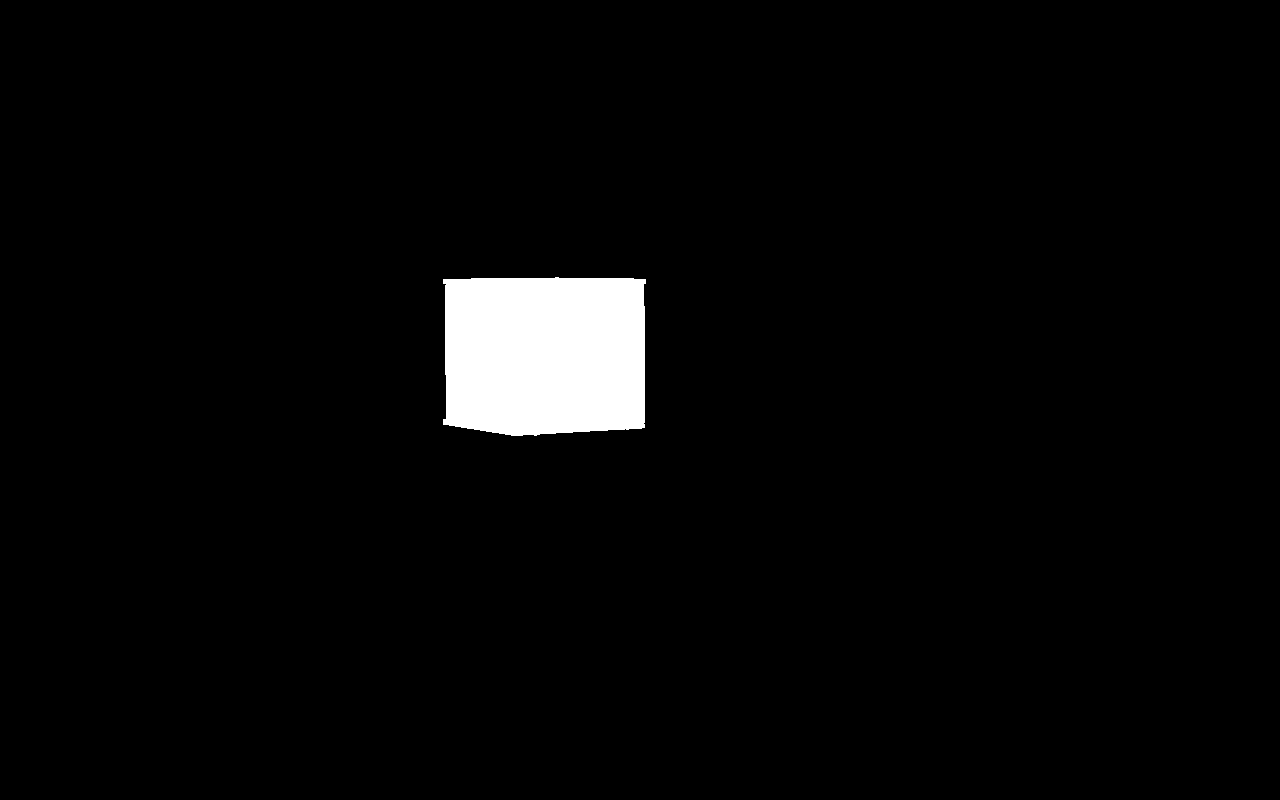
\includegraphics[scale=0.07]{good_examples/visual_211770_w_np.png}
\end{subfigure}
\begin{subfigure}[t]{0.19\textwidth}
\centering
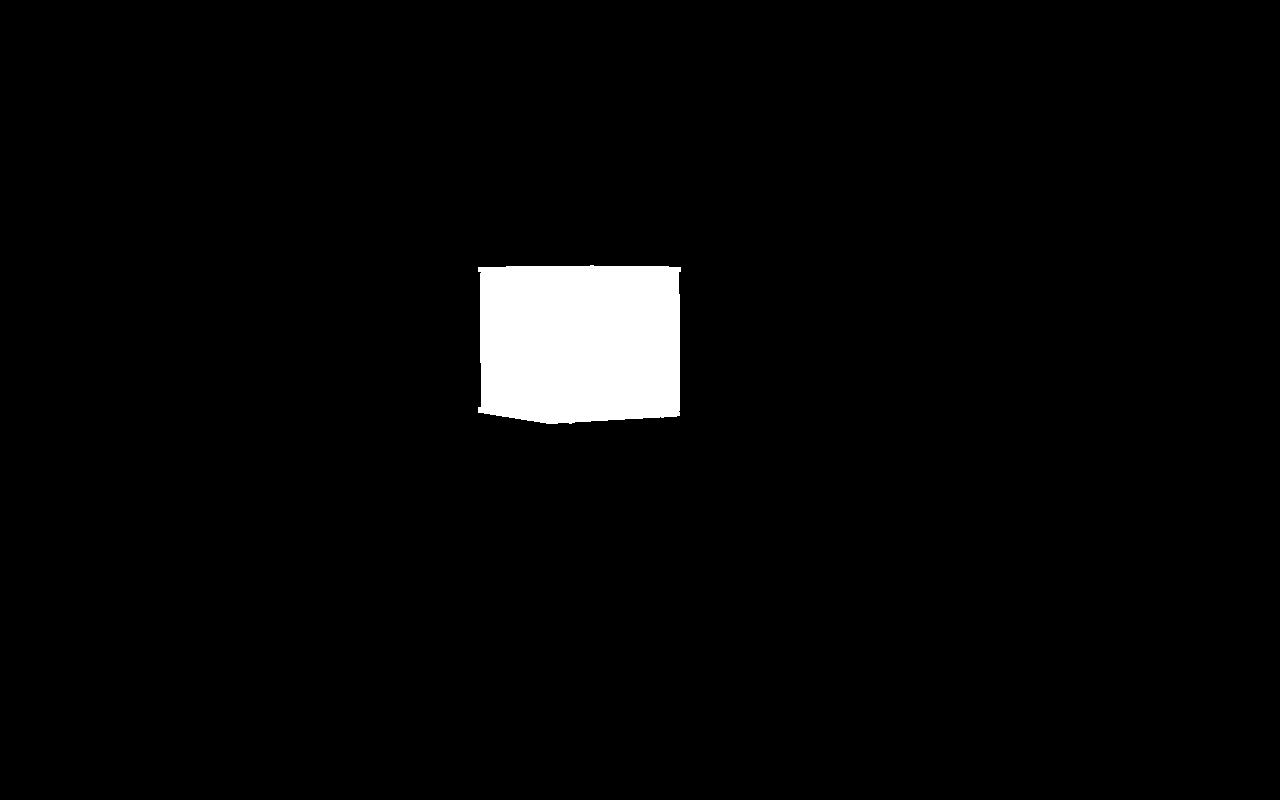
\includegraphics[scale=0.07]{good_examples/visual_211770_wo_np.png}
\end{subfigure}
\caption{IOU with reprojection: 0.94, IOU without reprojection: 0.65, video\_name: fbi\_2\_ext, frame\_number: 278.}
\end{figure}
\begin{figure}
\centering
\begin{subfigure}[t]{0.19\textwidth}
\centering
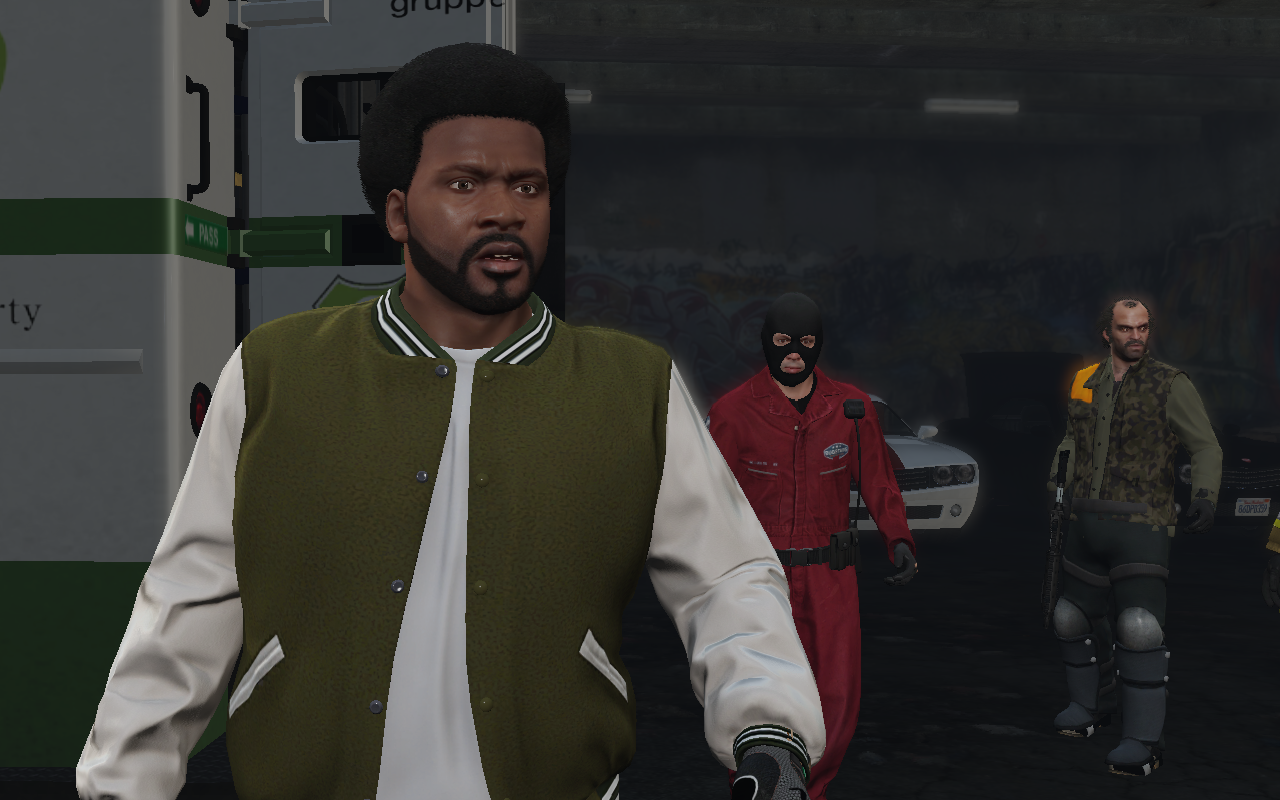
\includegraphics[scale=0.07]{good_examples/visual_29224_img.png}
\end{subfigure}
\begin{subfigure}[t]{0.19\textwidth}
\centering

\includegraphics[scale=0.07]{good_examples/visual_29224_img1.png}
\end{subfigure}
\begin{subfigure}[t]{0.19\textwidth}
\centering
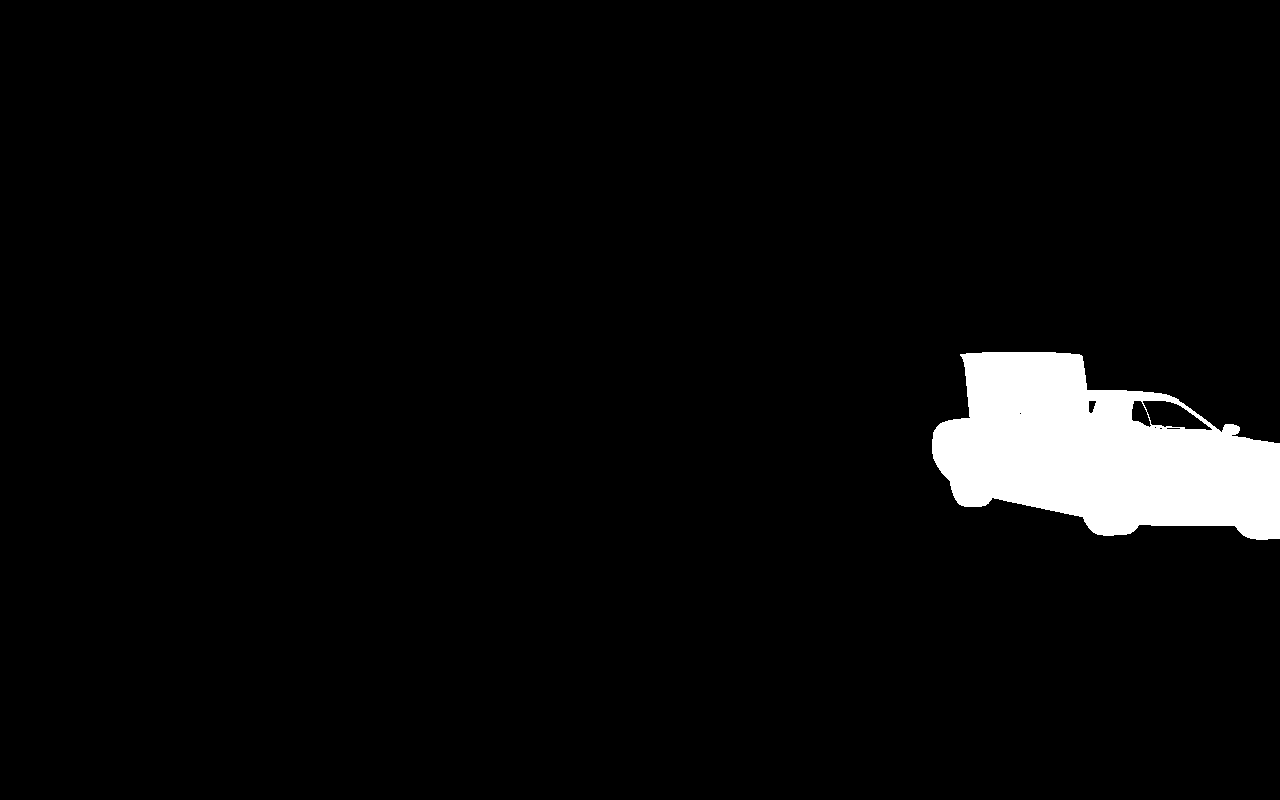
\includegraphics[scale=0.07]{good_examples/visual_29224_gt.png}
\end{subfigure}
\begin{subfigure}[t]{0.19\textwidth}
\centering
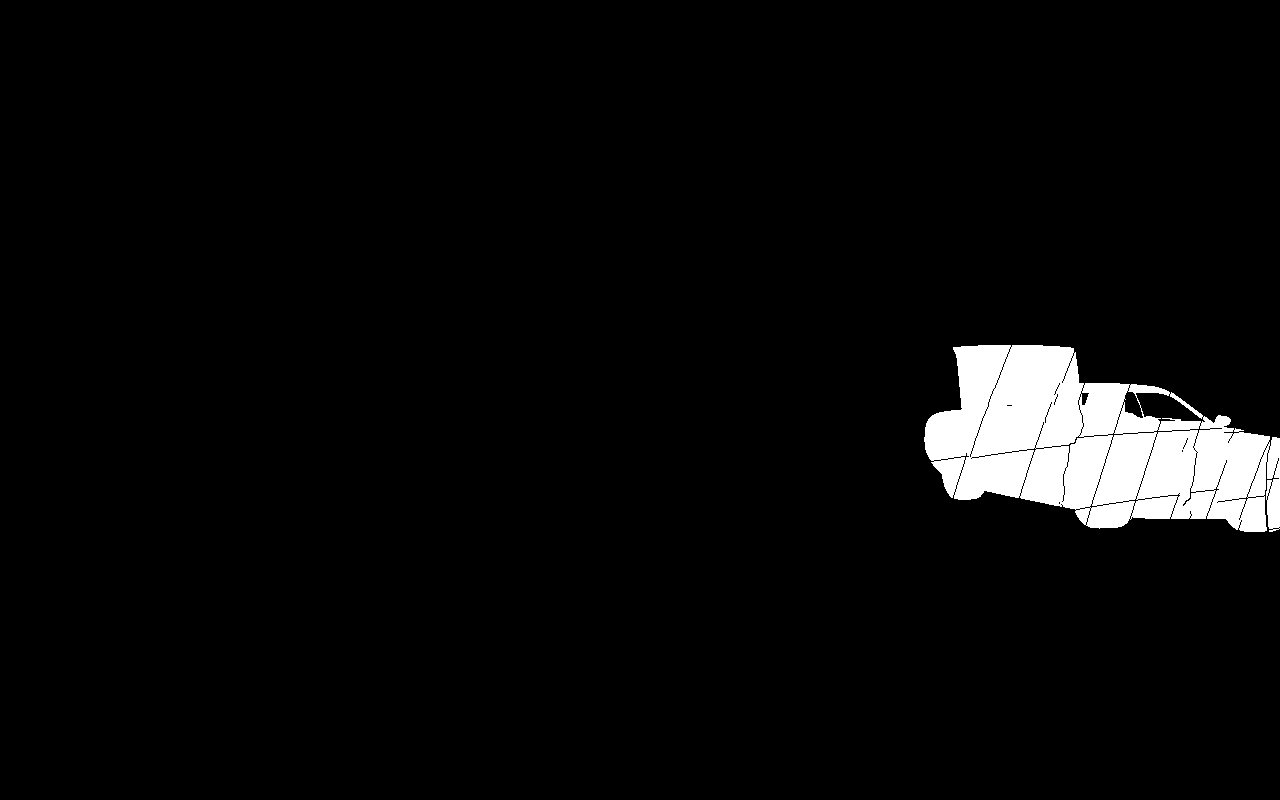
\includegraphics[scale=0.07]{good_examples/visual_29224_w_np.png}
\end{subfigure}
\begin{subfigure}[t]{0.19\textwidth}
\centering
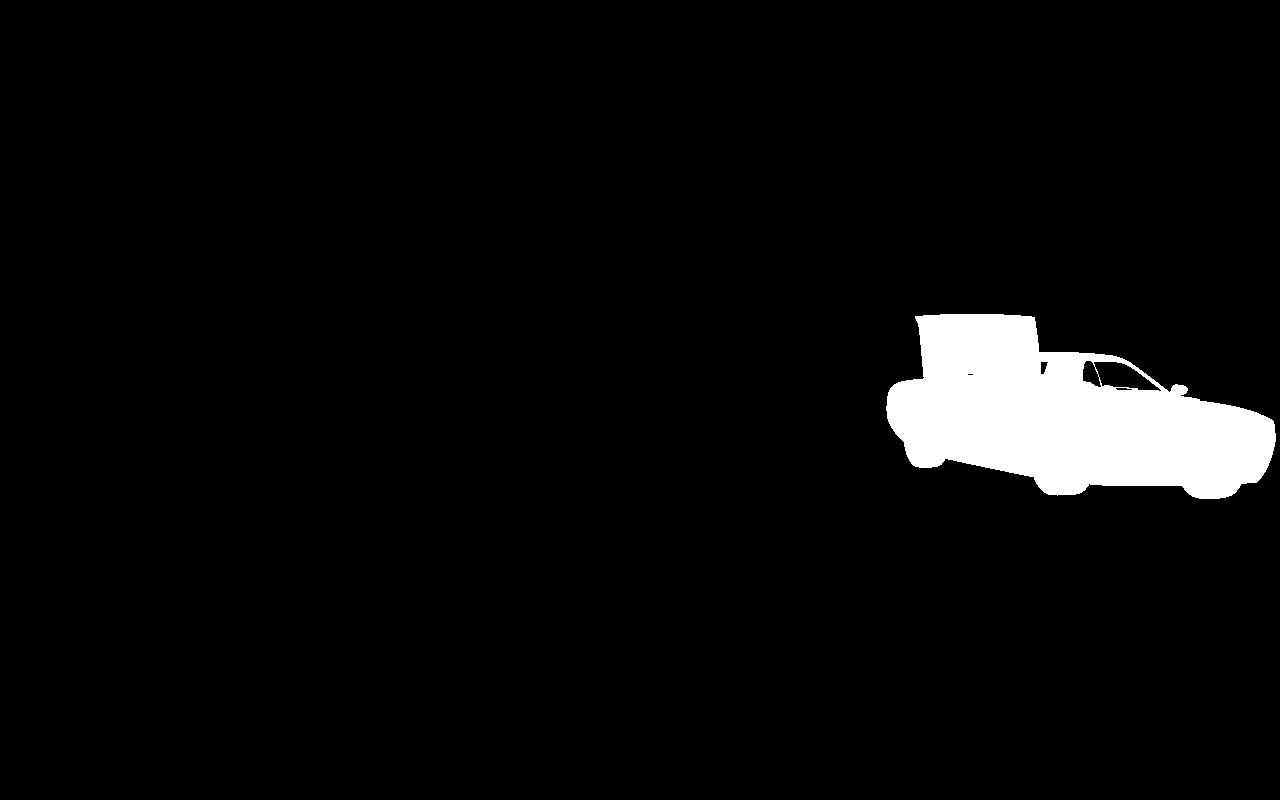
\includegraphics[scale=0.07]{good_examples/visual_29224_wo_np.png}
\end{subfigure}
\caption{IOU with reprojection: 0.82, IOU without reprojection: 0.51, video\_name: bs\_2a\_mcs\_8, frame\_number: 498.}
\end{figure}

\begin{figure}
\centering
\begin{subfigure}[t]{0.19\textwidth}
\centering
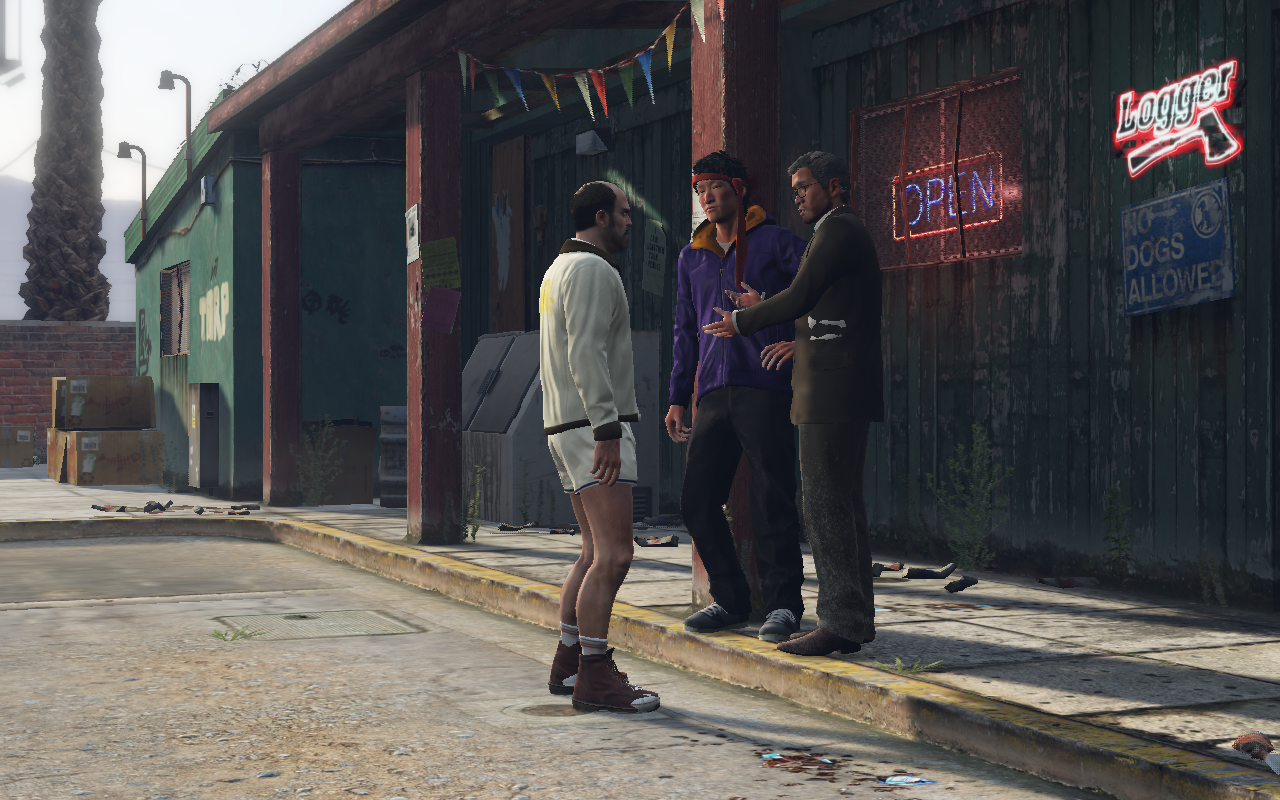
\includegraphics[scale=0.07]{good_examples/visual_81815_img.png}
\end{subfigure}
\begin{subfigure}[t]{0.19\textwidth}
\centering
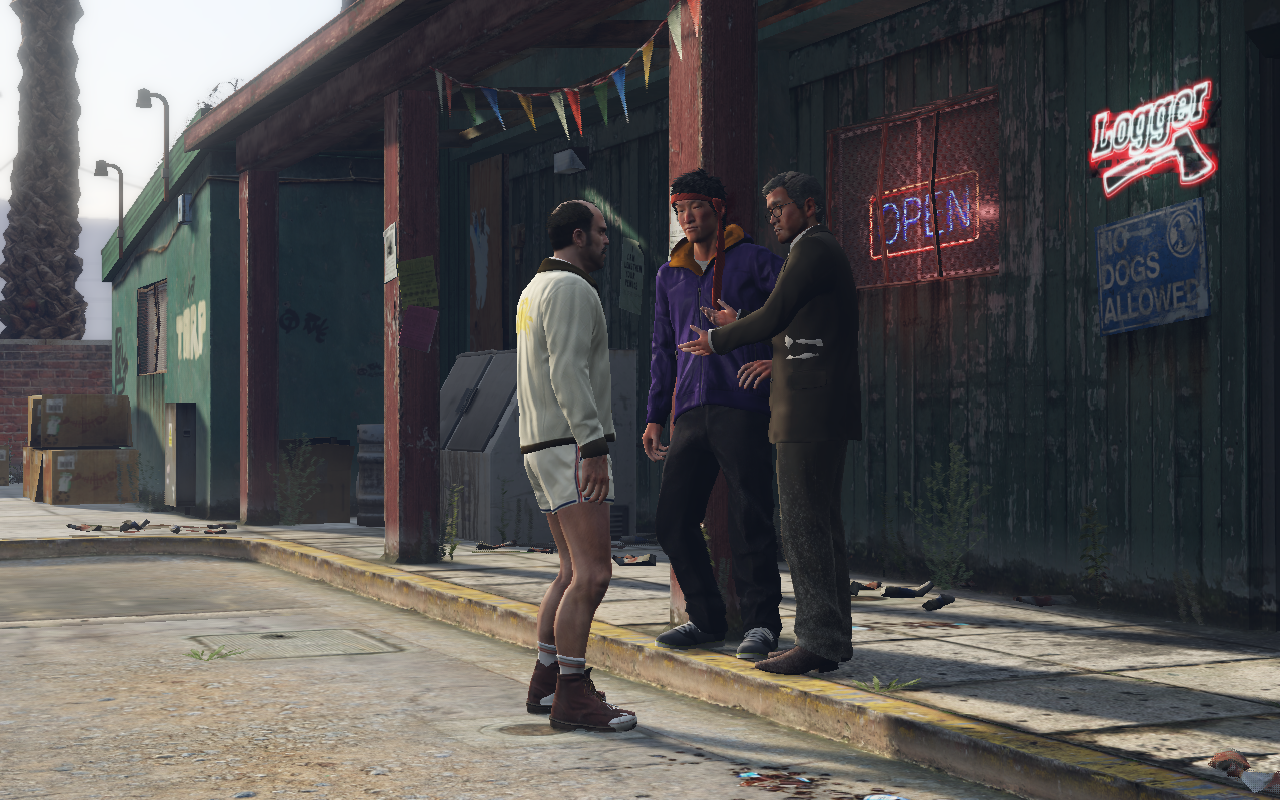
\includegraphics[scale=0.07]{good_examples/visual_81815_img1.png}
\end{subfigure}
\begin{subfigure}[t]{0.19\textwidth}
\centering
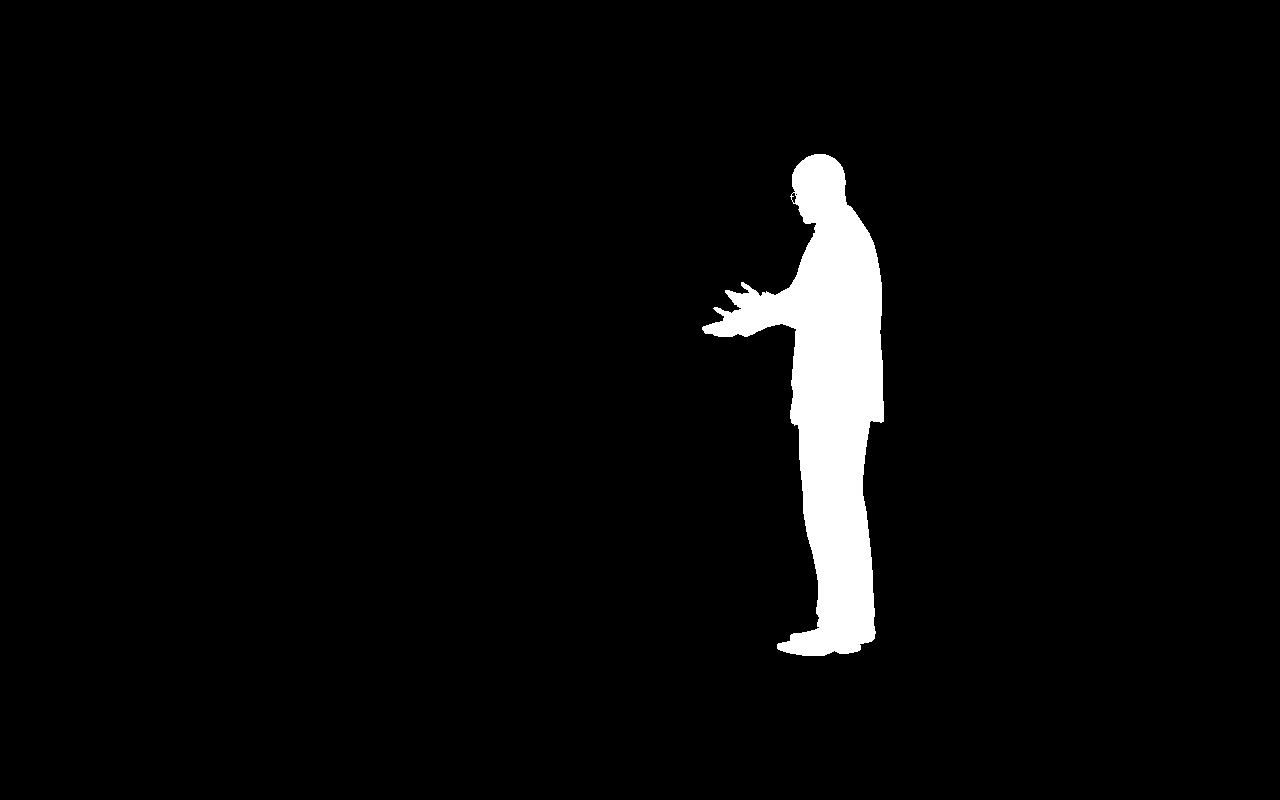
\includegraphics[scale=0.07]{good_examples/visual_81815_gt.png}
\end{subfigure}
\begin{subfigure}[t]{0.19\textwidth}
\centering
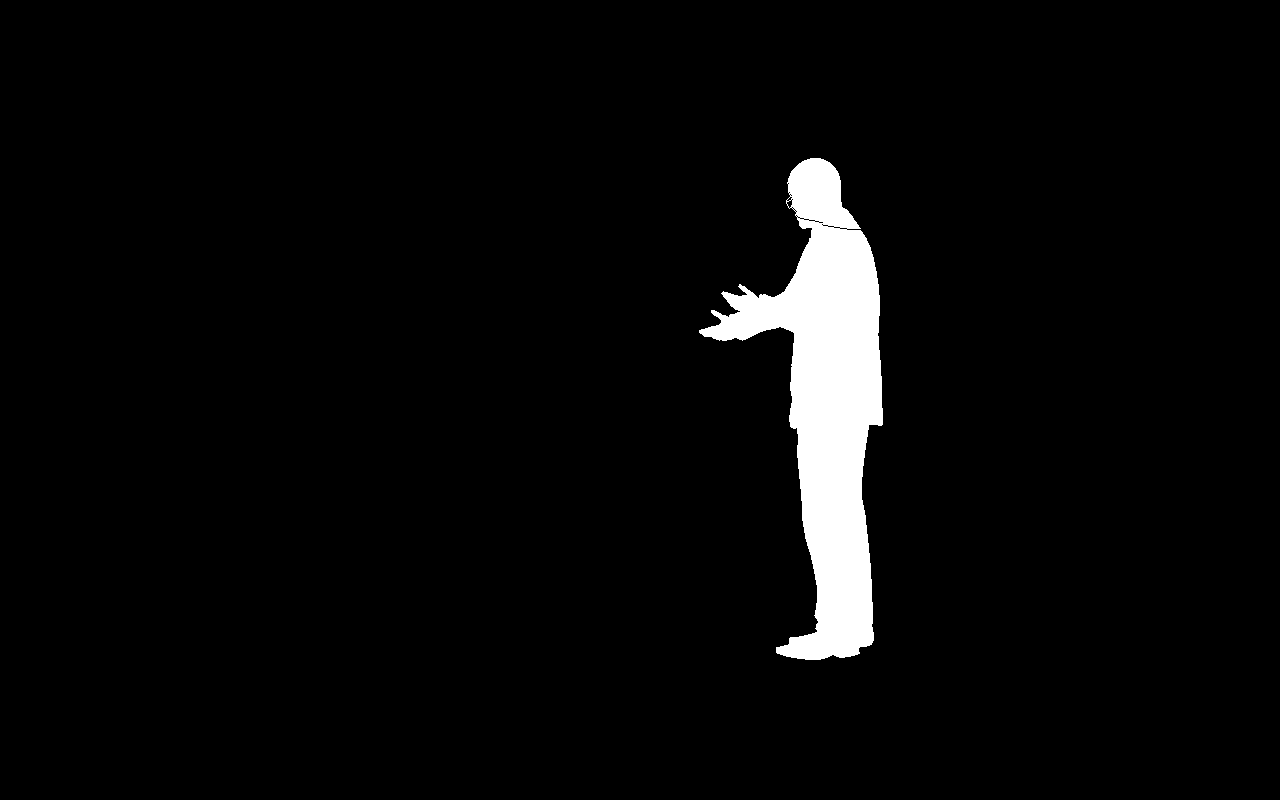
\includegraphics[scale=0.07]{good_examples/visual_81815_w_np.png}
\end{subfigure}
\begin{subfigure}[t]{0.19\textwidth}
\centering
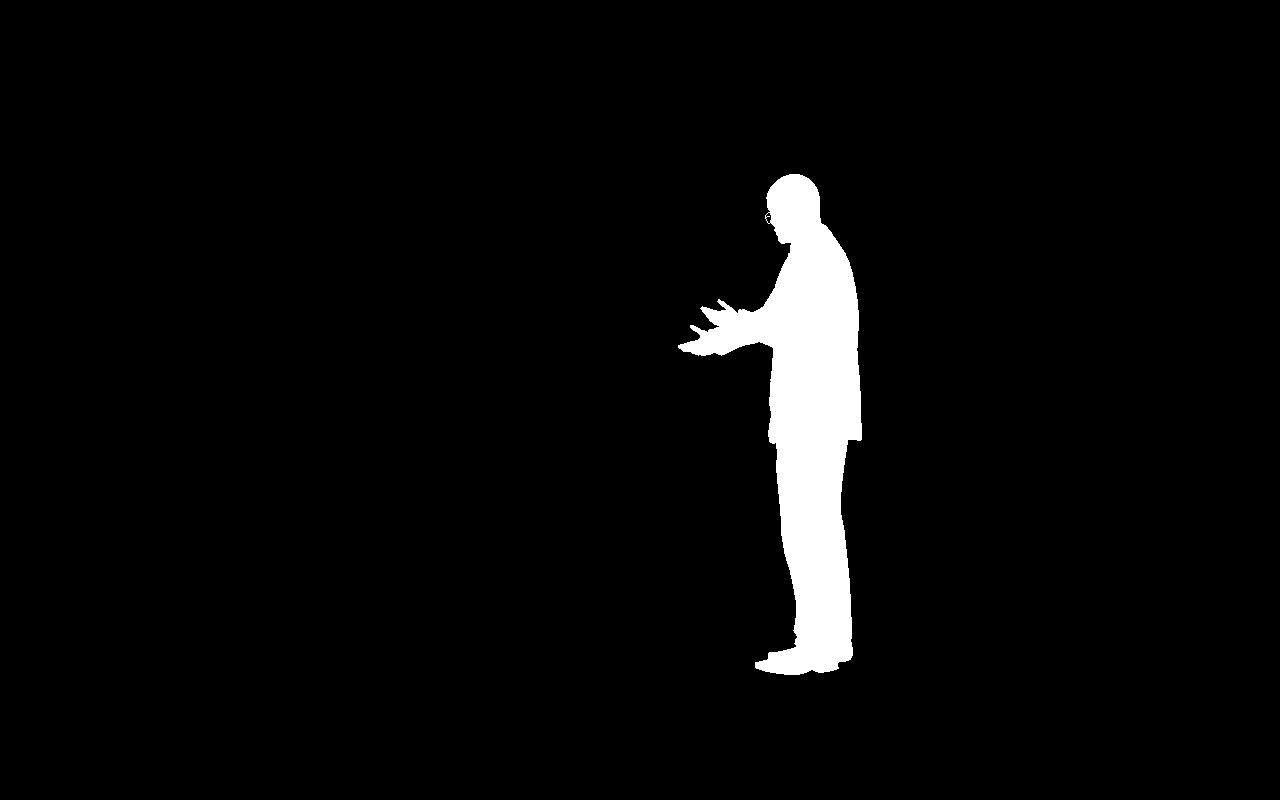
\includegraphics[scale=0.07]{good_examples/visual_81815_wo_np.png}
\end{subfigure}
\caption{IOU with reprojection: 0.90, IOU without reprojection: 0.47, video\_name: chinese\_2\_int, frame\_number: 456.}
\end{figure}

\begin{figure}
\centering
\begin{subfigure}[t]{0.19\textwidth}
\centering
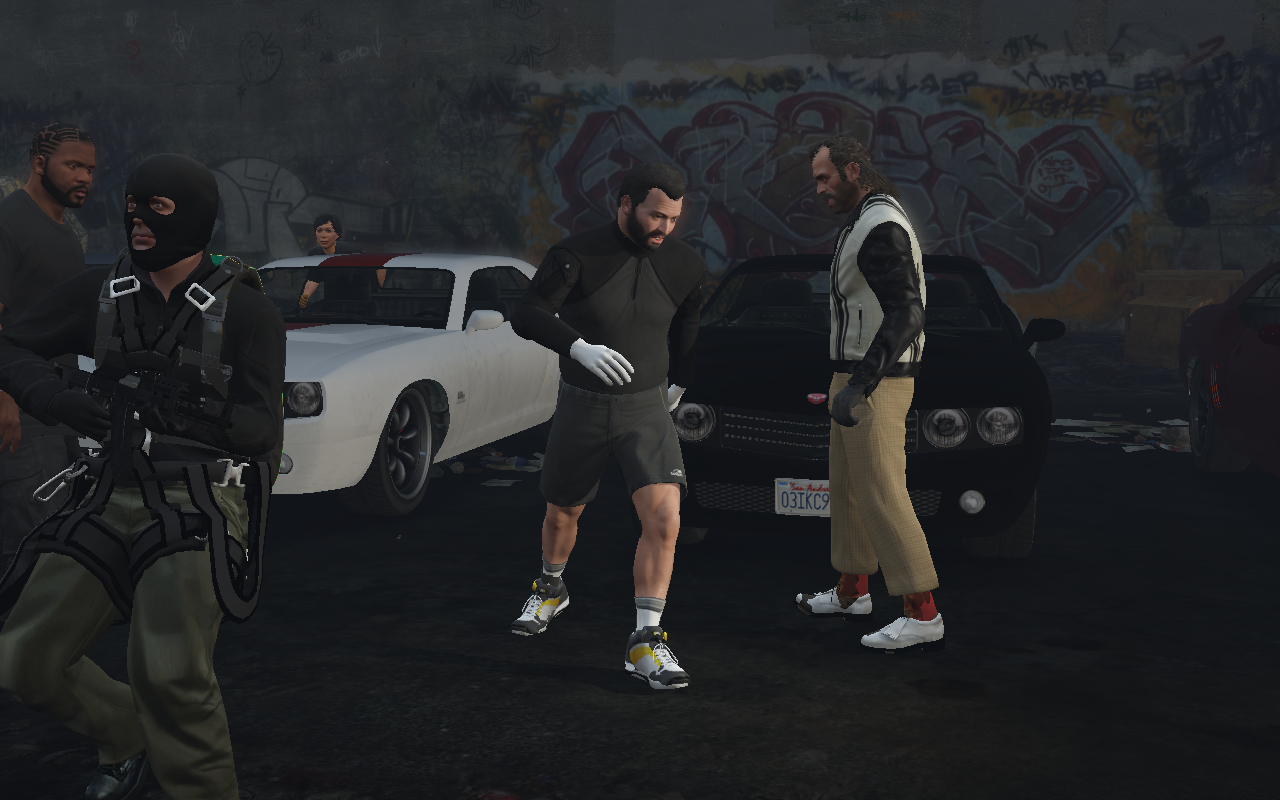
\includegraphics[scale=0.07]{good_examples/visual_34430_img.png}
\end{subfigure}
\begin{subfigure}[t]{0.19\textwidth}
\centering
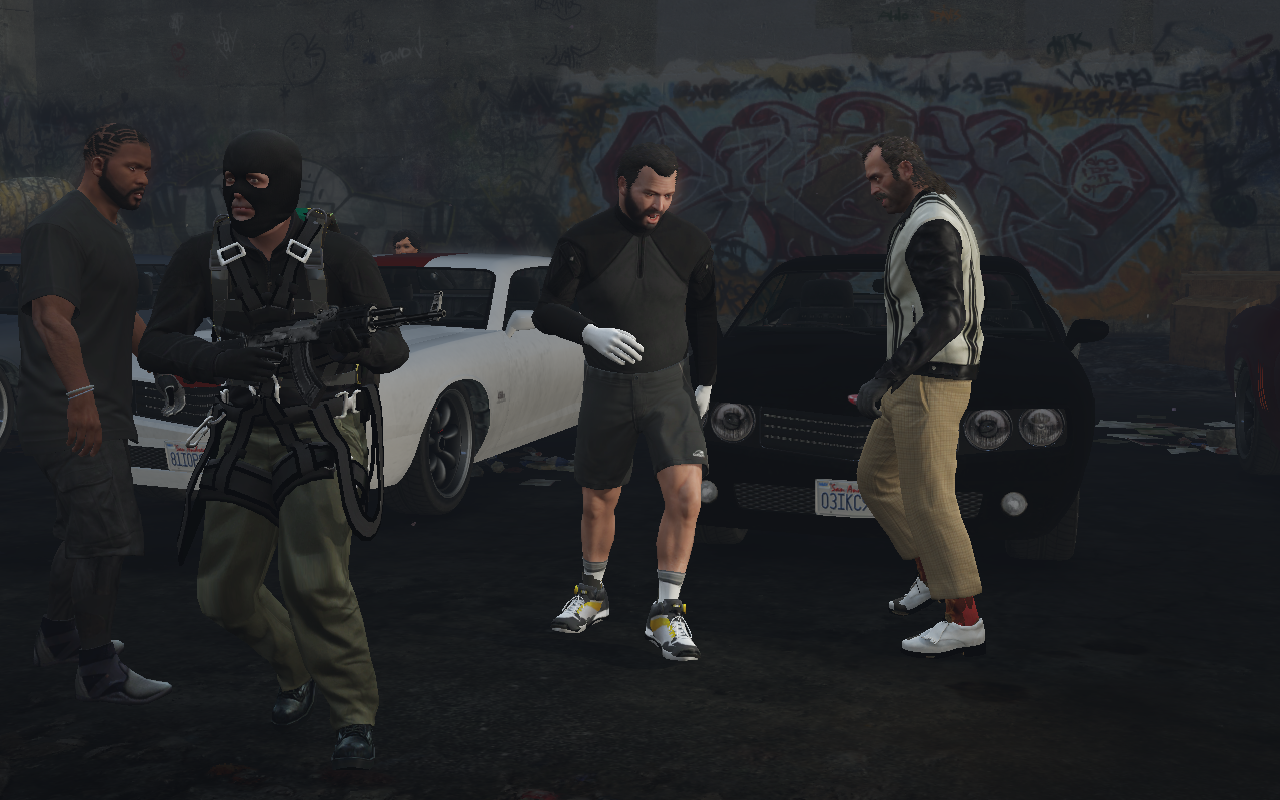
\includegraphics[scale=0.07]{good_examples/visual_34430_img1.png}
\end{subfigure}
\begin{subfigure}[t]{0.19\textwidth}
\centering
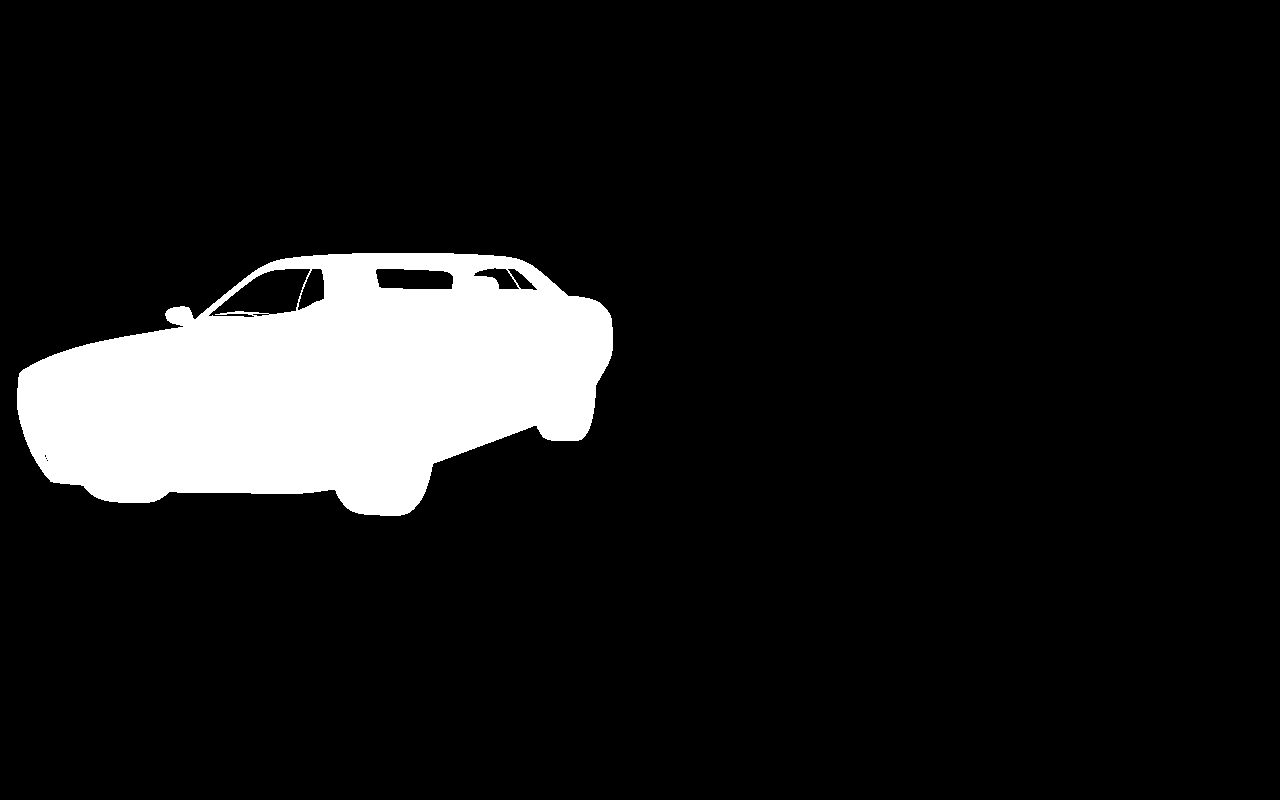
\includegraphics[scale=0.07]{good_examples/visual_34430_gt.png}
\end{subfigure}
\begin{subfigure}[t]{0.19\textwidth}
\centering
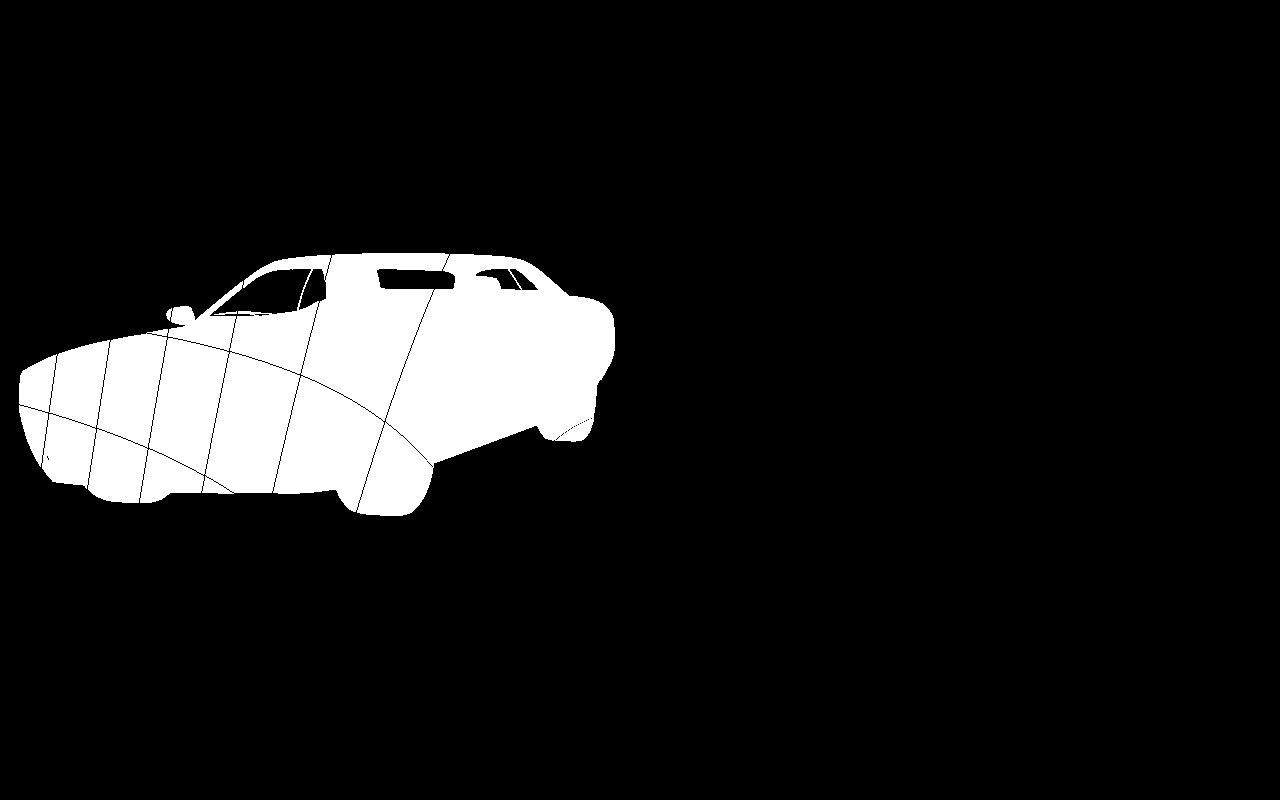
\includegraphics[scale=0.07]{good_examples/visual_34430_w_np.png}
\end{subfigure}
\begin{subfigure}[t]{0.19\textwidth}
\centering
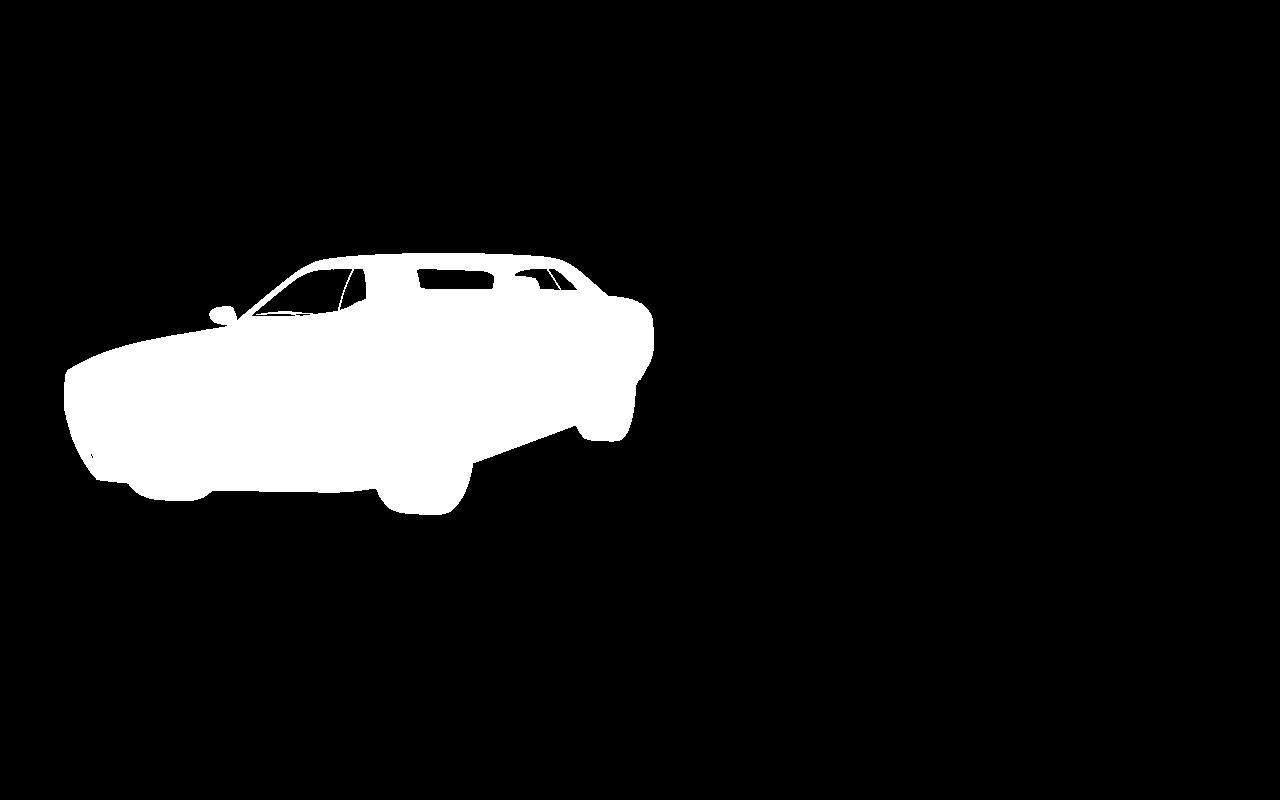
\includegraphics[scale=0.07]{good_examples/visual_34430_wo_np.png}
\end{subfigure}
\caption{IOU with reprojection: 0.97, IOU without reprojection: 0.76, video\_name: bs\_2a\_mcs\_8\_p3, frame\_number: 79.}
\end{figure}

\begin{figure}
\centering
\begin{subfigure}[t]{0.19\textwidth}
\centering
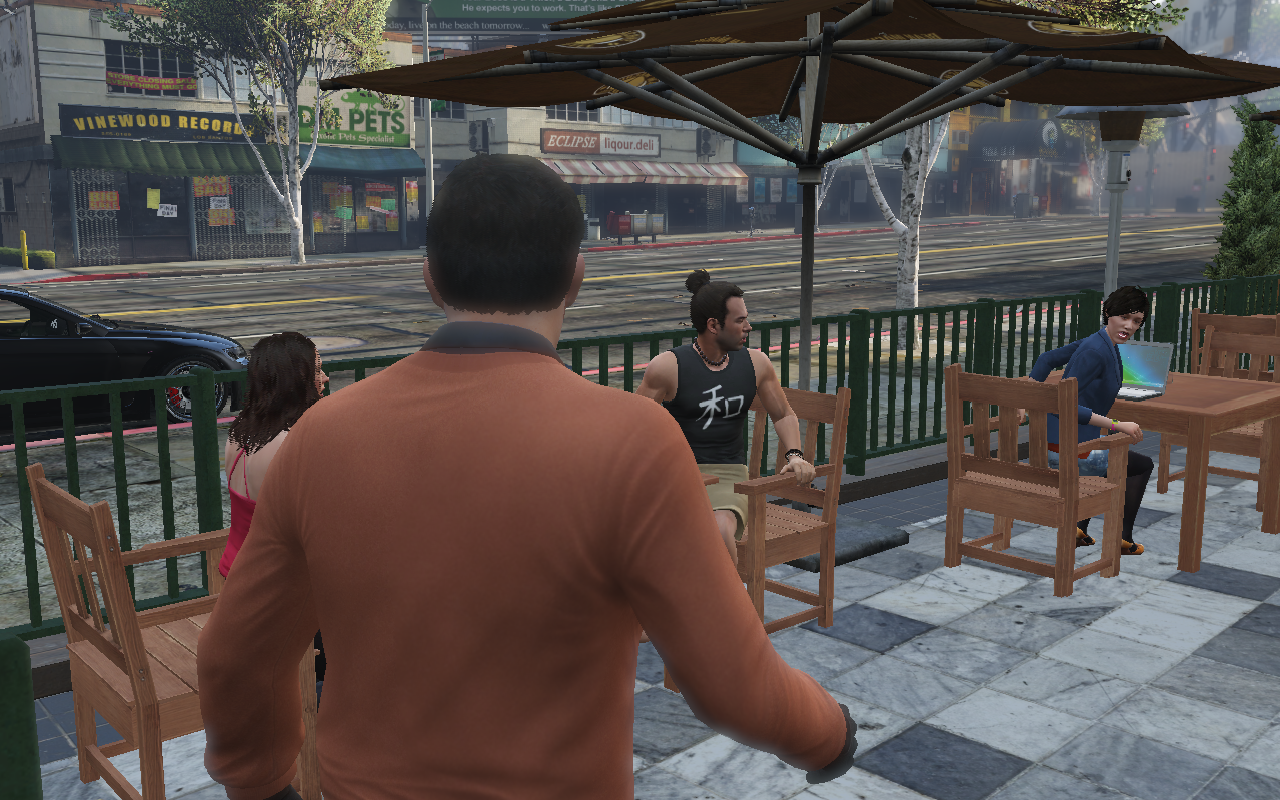
\includegraphics[scale=0.07]{good_examples/visual_99358_img.png}
\end{subfigure}
\begin{subfigure}[t]{0.19\textwidth}
\centering
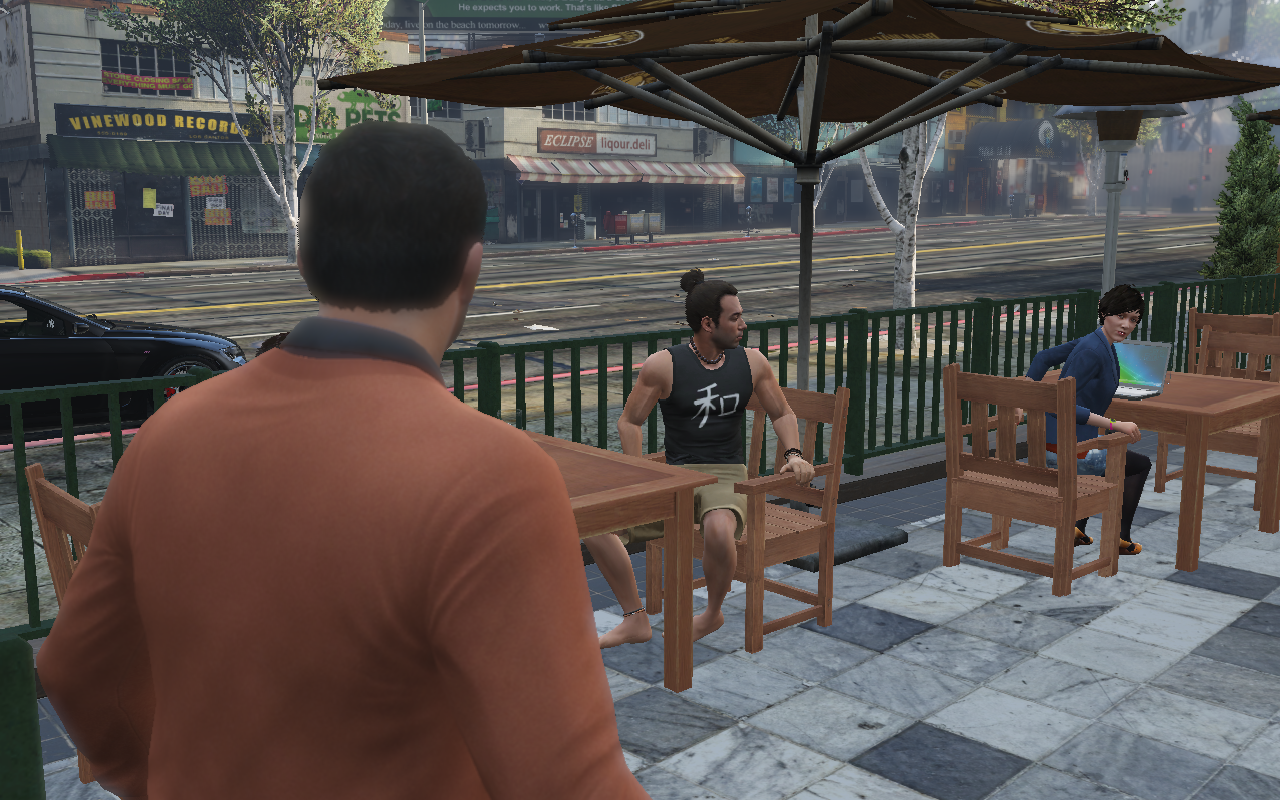
\includegraphics[scale=0.07]{good_examples/visual_99358_img1.png}
\end{subfigure}
\begin{subfigure}[t]{0.19\textwidth}
\centering
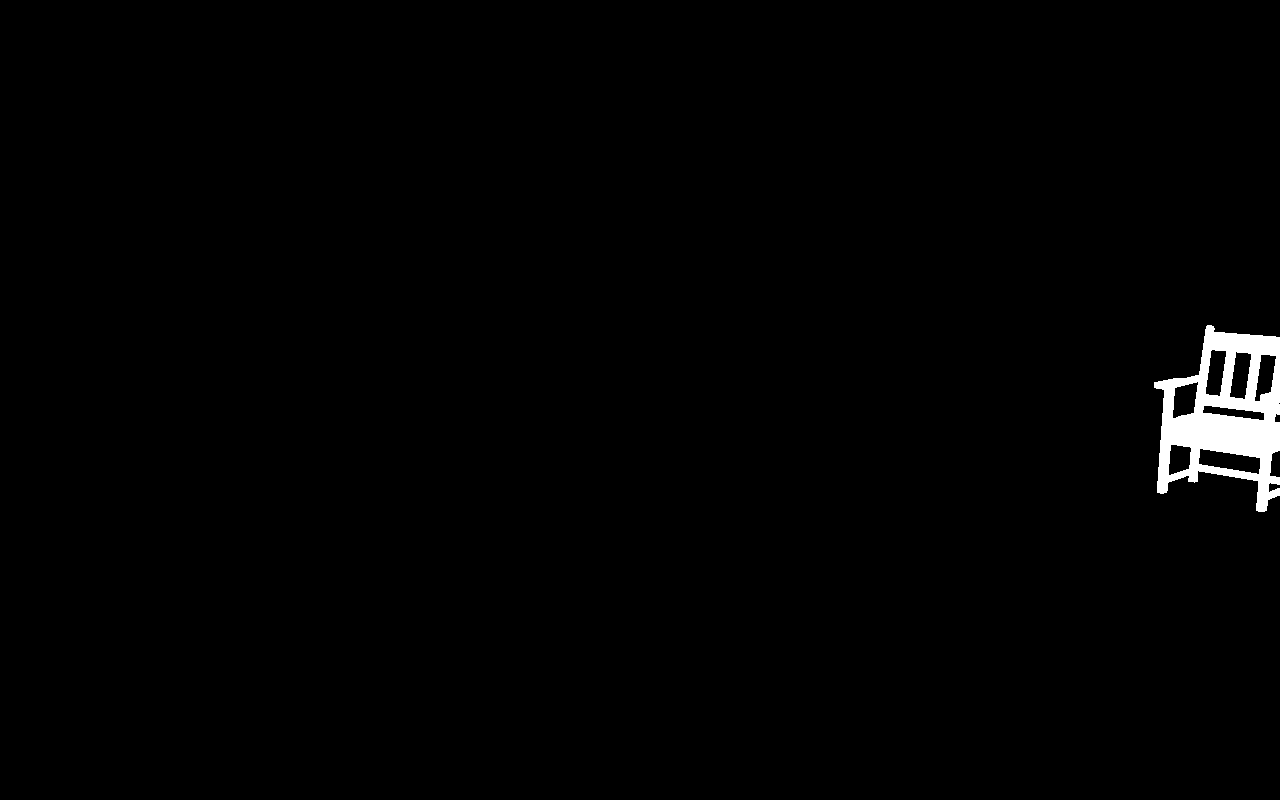
\includegraphics[scale=0.07]{good_examples/visual_99358_gt.png}
\end{subfigure}
\begin{subfigure}[t]{0.19\textwidth}
\centering
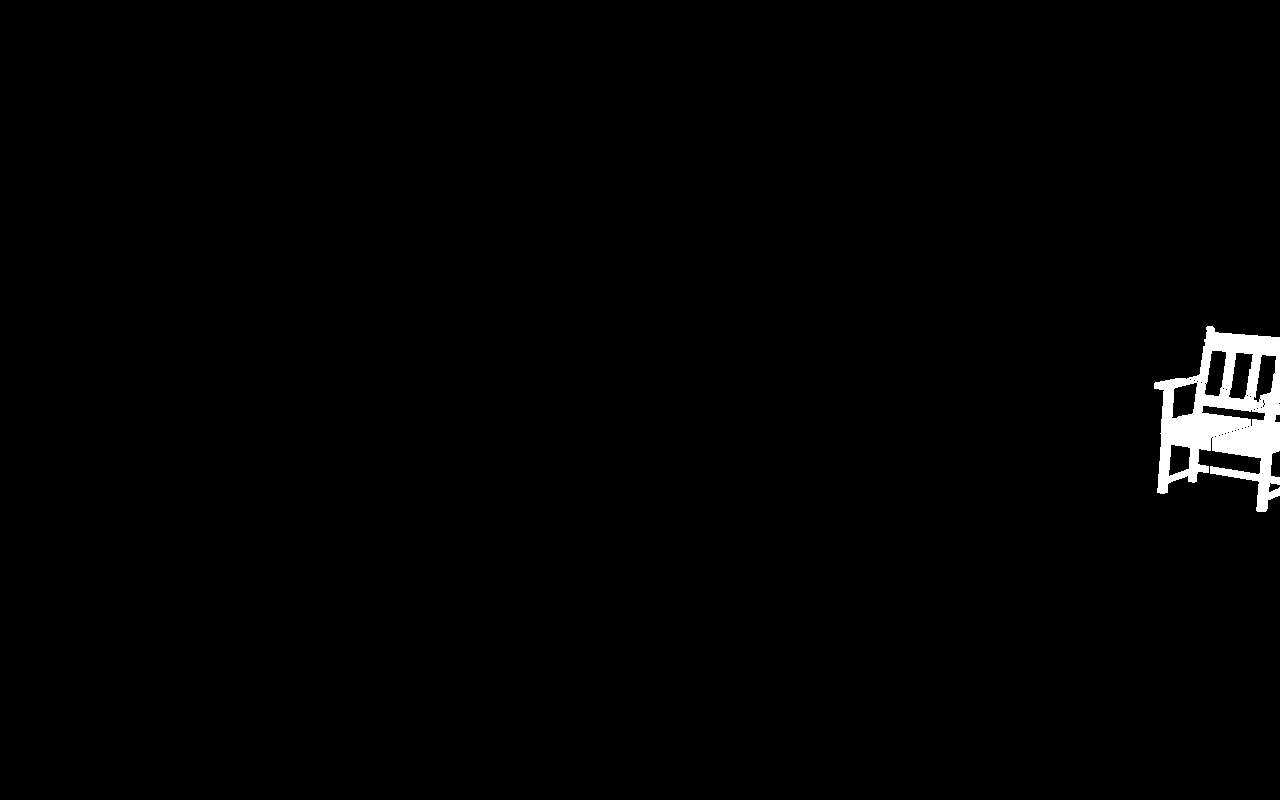
\includegraphics[scale=0.07]{good_examples/visual_99358_w_np.png}
\end{subfigure}
\begin{subfigure}[t]{0.19\textwidth}
\centering
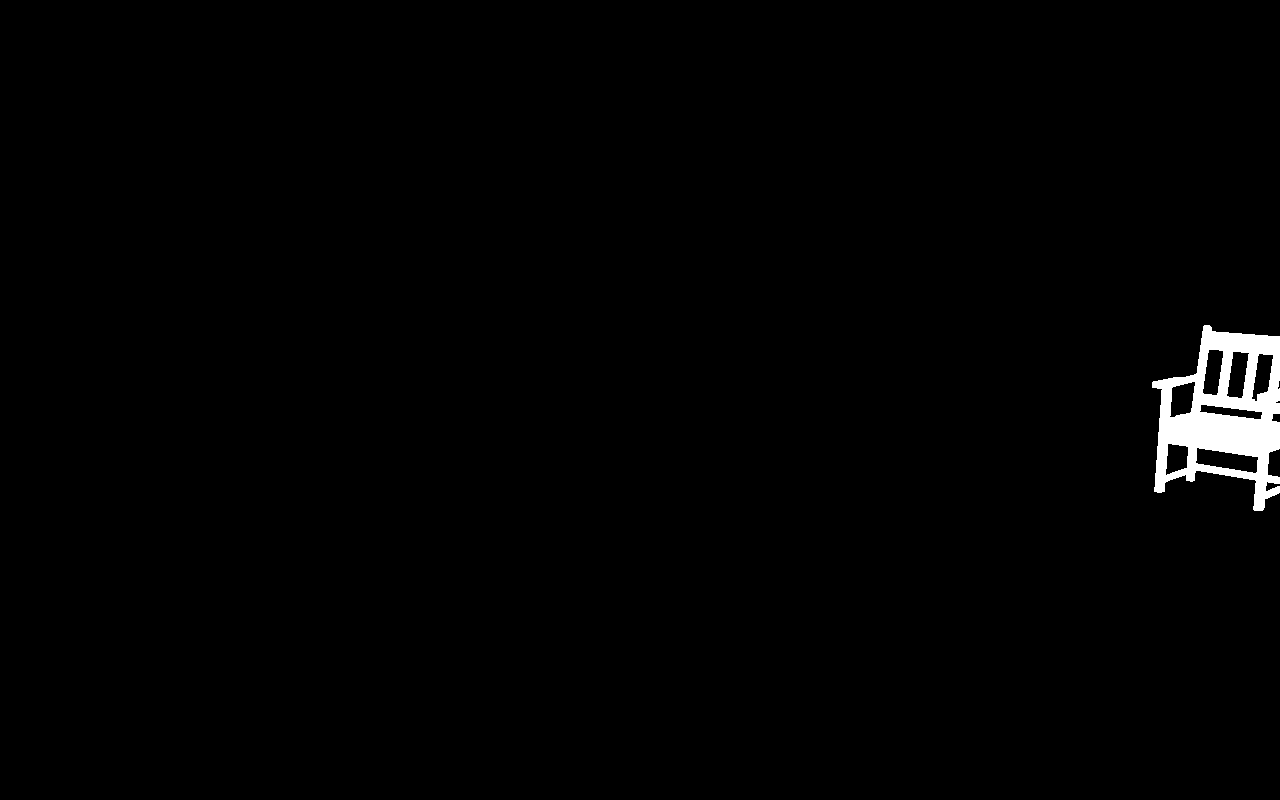
\includegraphics[scale=0.07]{good_examples/visual_99358_wo_np.png}
\end{subfigure}
\caption{IOU with reprojection: 0.94, IOU without reprojection: 0.81, video\_name: fam\_6\_mcs\_1, frame\_number: 25.}
\end{figure}

\begin{figure}
\centering
\begin{subfigure}[t]{0.19\textwidth}
\centering

\includegraphics[scale=0.07]{good_examples/visual_69756_img.png}
\end{subfigure}
\begin{subfigure}[t]{0.19\textwidth}
\centering

\includegraphics[scale=0.07]{good_examples/visual_69756_img1.png}
\end{subfigure}
\begin{subfigure}[t]{0.19\textwidth}
\centering
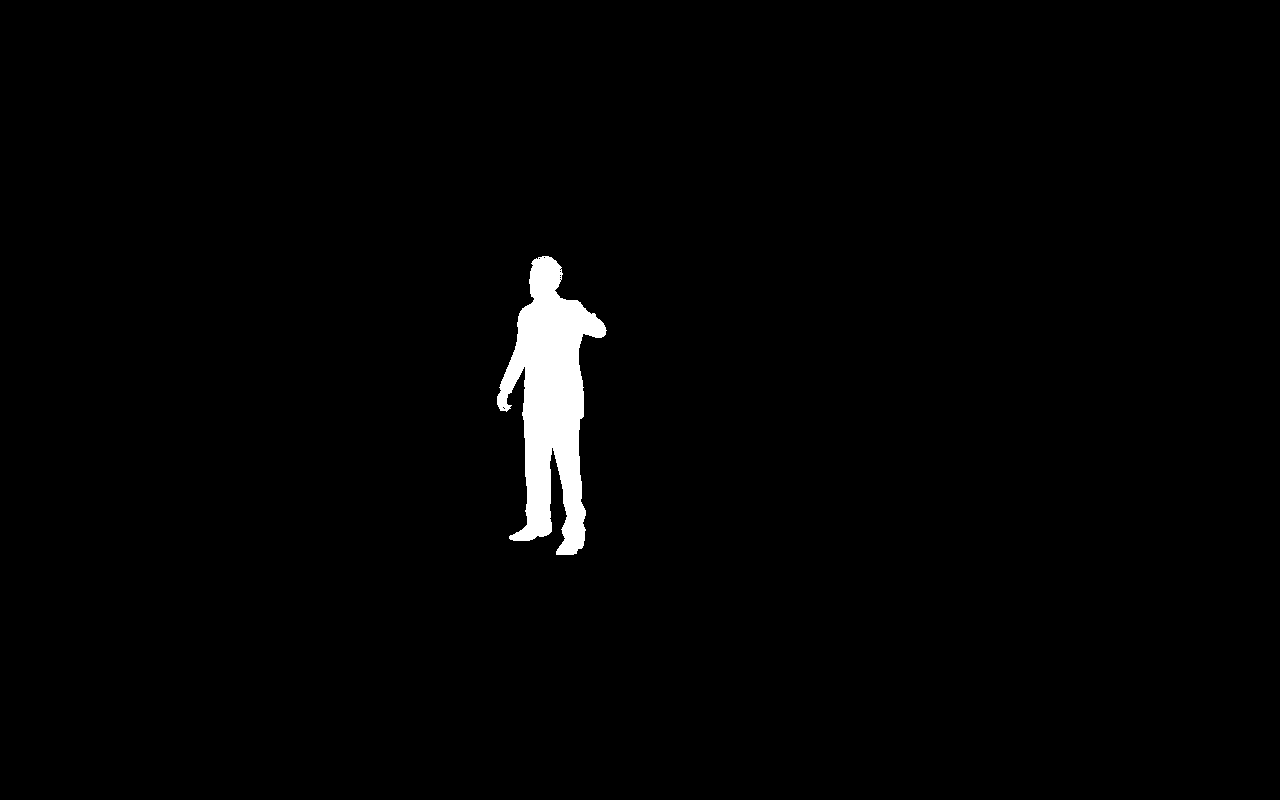
\includegraphics[scale=0.07]{good_examples/visual_69756_gt.png}
\end{subfigure}
\begin{subfigure}[t]{0.19\textwidth}
\centering
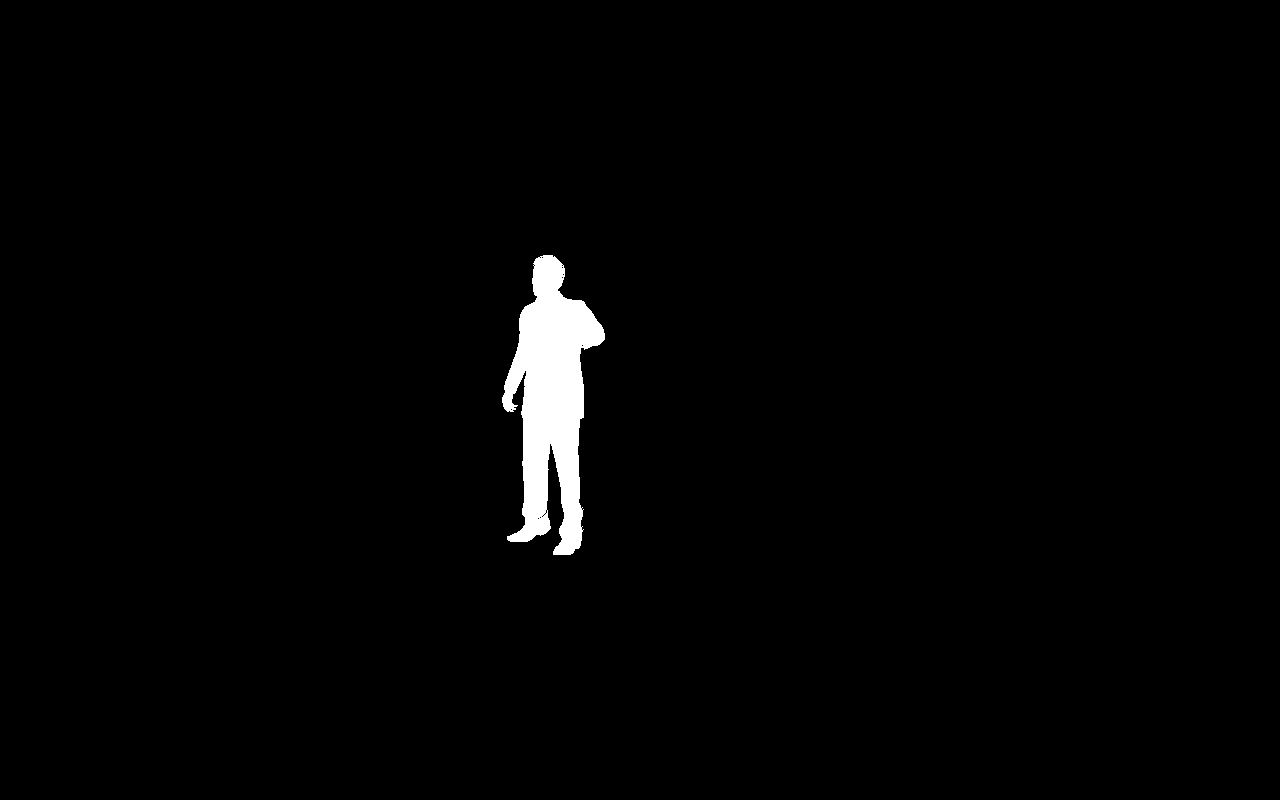
\includegraphics[scale=0.07]{good_examples/visual_69756_w_np.png}
\end{subfigure}
\begin{subfigure}[t]{0.19\textwidth}
\centering
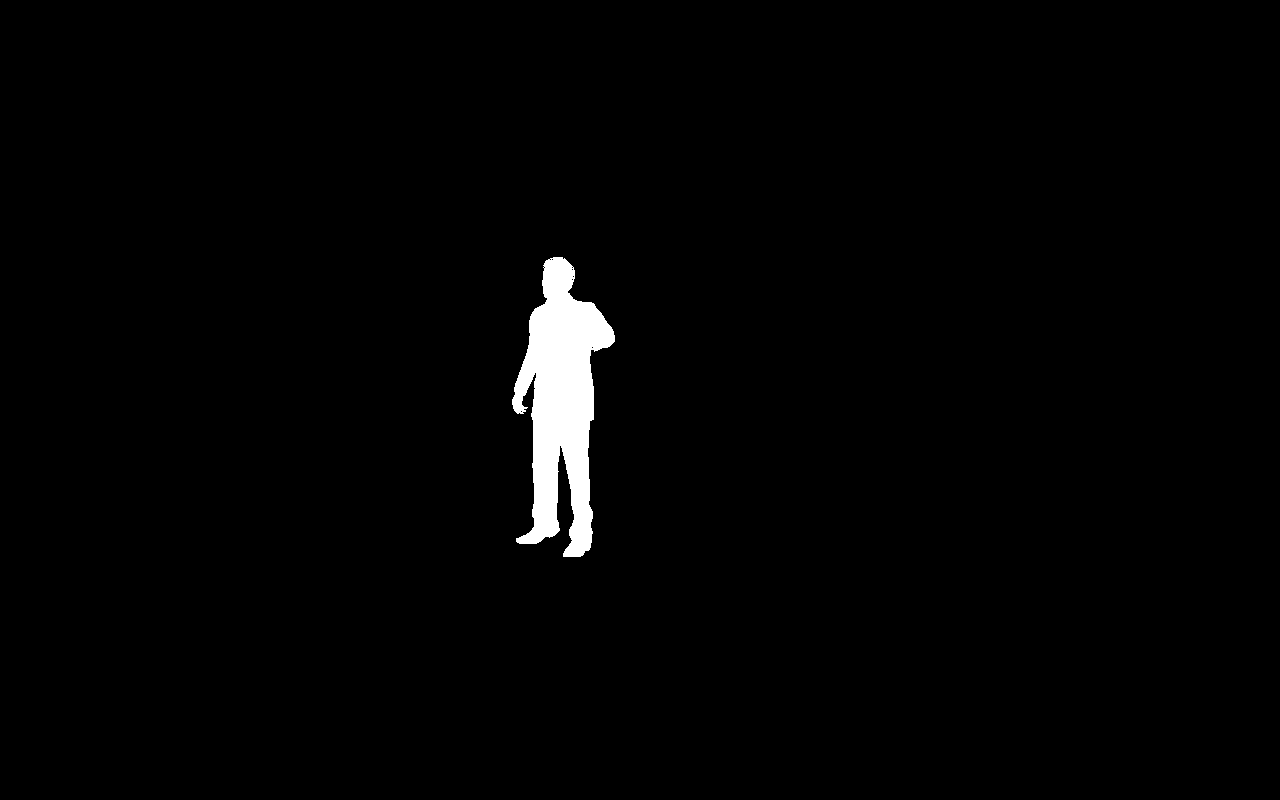
\includegraphics[scale=0.07]{good_examples/visual_69756_wo_np.png}
\end{subfigure}
\caption{IOU with reprojection: 0.87, IOU without reprojection: 0.59, video\_name: chinese\_1\_int, frame\_number: 550.}
\end{figure}




\begin{figure}
\centering
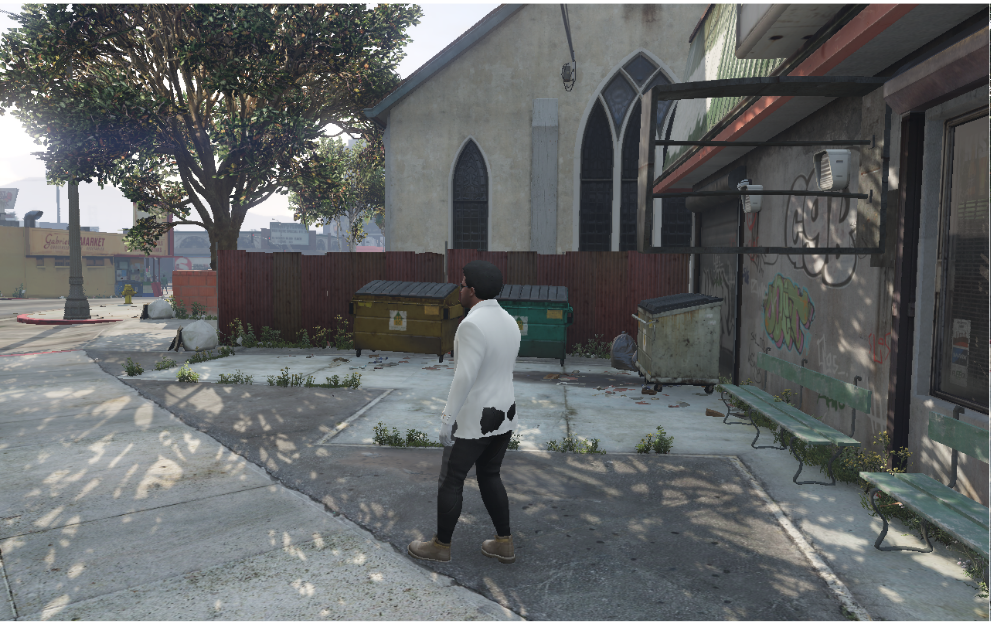
\includegraphics[scale=0.2]{fig/270i.png}
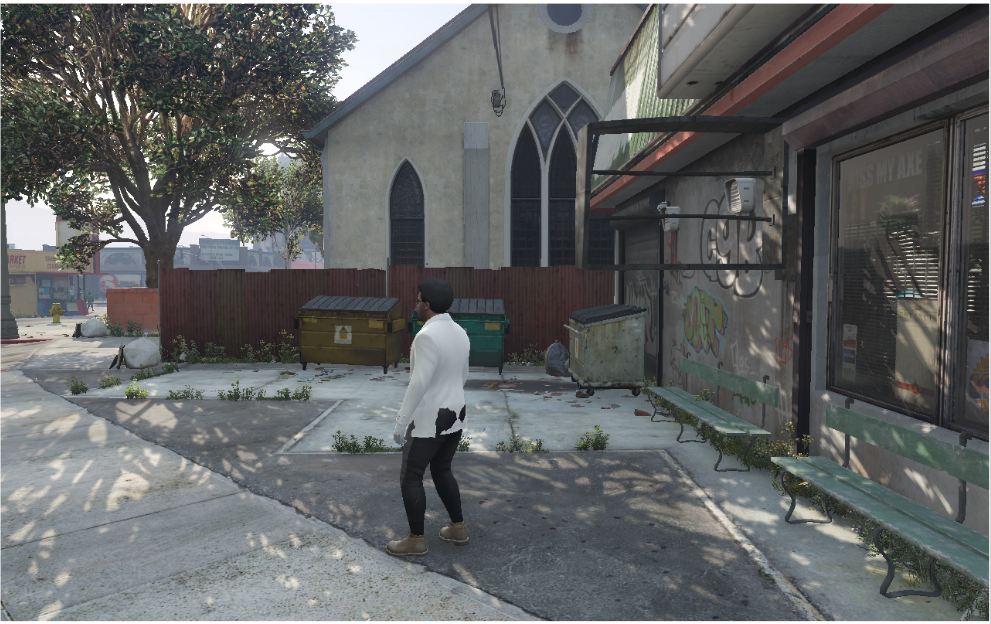
\includegraphics[scale=0.2]{fig/271i.png}
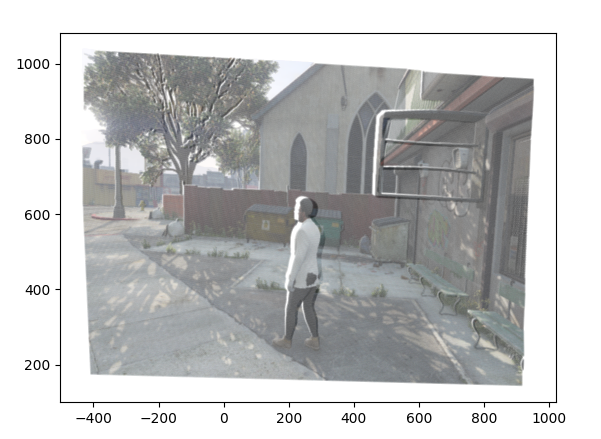
\includegraphics[scale=0.38]{fig/270r271.png}
\caption{Image from SAILVOS dataset video \text{tonya\_concat\_1} frame 270 and 271. The third figure is the result of reproject frame 270 to the view of 271. We can see that the camera moved left from frame 270 to 271, which is reflected in the reprojected image.}
\label{fig:reproj_image}
\end{figure}